\documentclass{article}
\usepackage{amsmath}   % for mathematical equations
\usepackage{graphicx}  % for including graphs and images
\usepackage{float}     % to force figure placement
\usepackage{caption}   % for figure captions
\usepackage{siunitx}   % for units formatting
\usepackage{hyperref}  % for links

\title{Lab Report III: Operational Amplifiers}
\author{Enrique Rivera \\ Lab Partner: Marcus}
\date{\today}

\begin{document}
\maketitle

\section*{Lab 7: Operational Amplifiers}

\subsection*{Objective}
The objective of this lab is to familiarize ourselves with the orientation 
and function of an op amp within a circuit and understand the two op-amp rules 
when building various amplifiers.

\subsection*{Question 1}
Recreate the circuit in Fig. 2 using an LM741CN op-amp. 
Breadboard setup with 
\( V_{CC} = 15.03 \, \text{V} \), \( V_{EE} = -15.08 \, \text{V} \), \( R_{g} = R_{in} = 10 \, \text{k}\Omega \). 
Set the waveform amplitude to \( 328 \, \text{mV} \) peak-to-peak.

\begin{figure}[H]
    \centering
    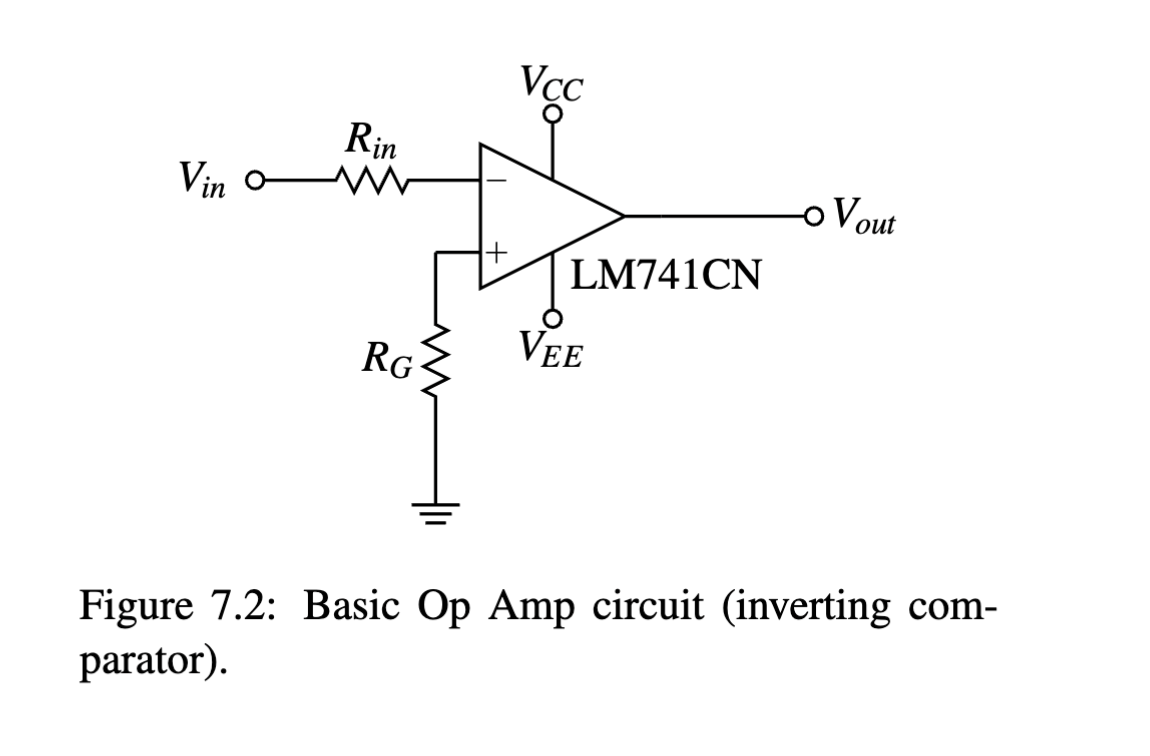
\includegraphics[width=0.8\textwidth]{img/Lab 7/1_1.png} 
    \caption{}
\end{figure}

When viewing our waveforms, we set our amplitude to be \( 160 \, \text{mV}_{\text{p.p.}} \), falling within the given
limits of \( 50 \, \text{mV} \) and \( 300 \, \text{mV} \). 
\\
Below are our observed waveforms in order of frequencies \( 135 \, \text{Hz} \), \( 1.35 \, \text{kHz} \), \( 4.2 \, \text{kHz} \), and
\( 25.05 \, \text{kHz} \).

\begin{figure}[H]
    \centering
    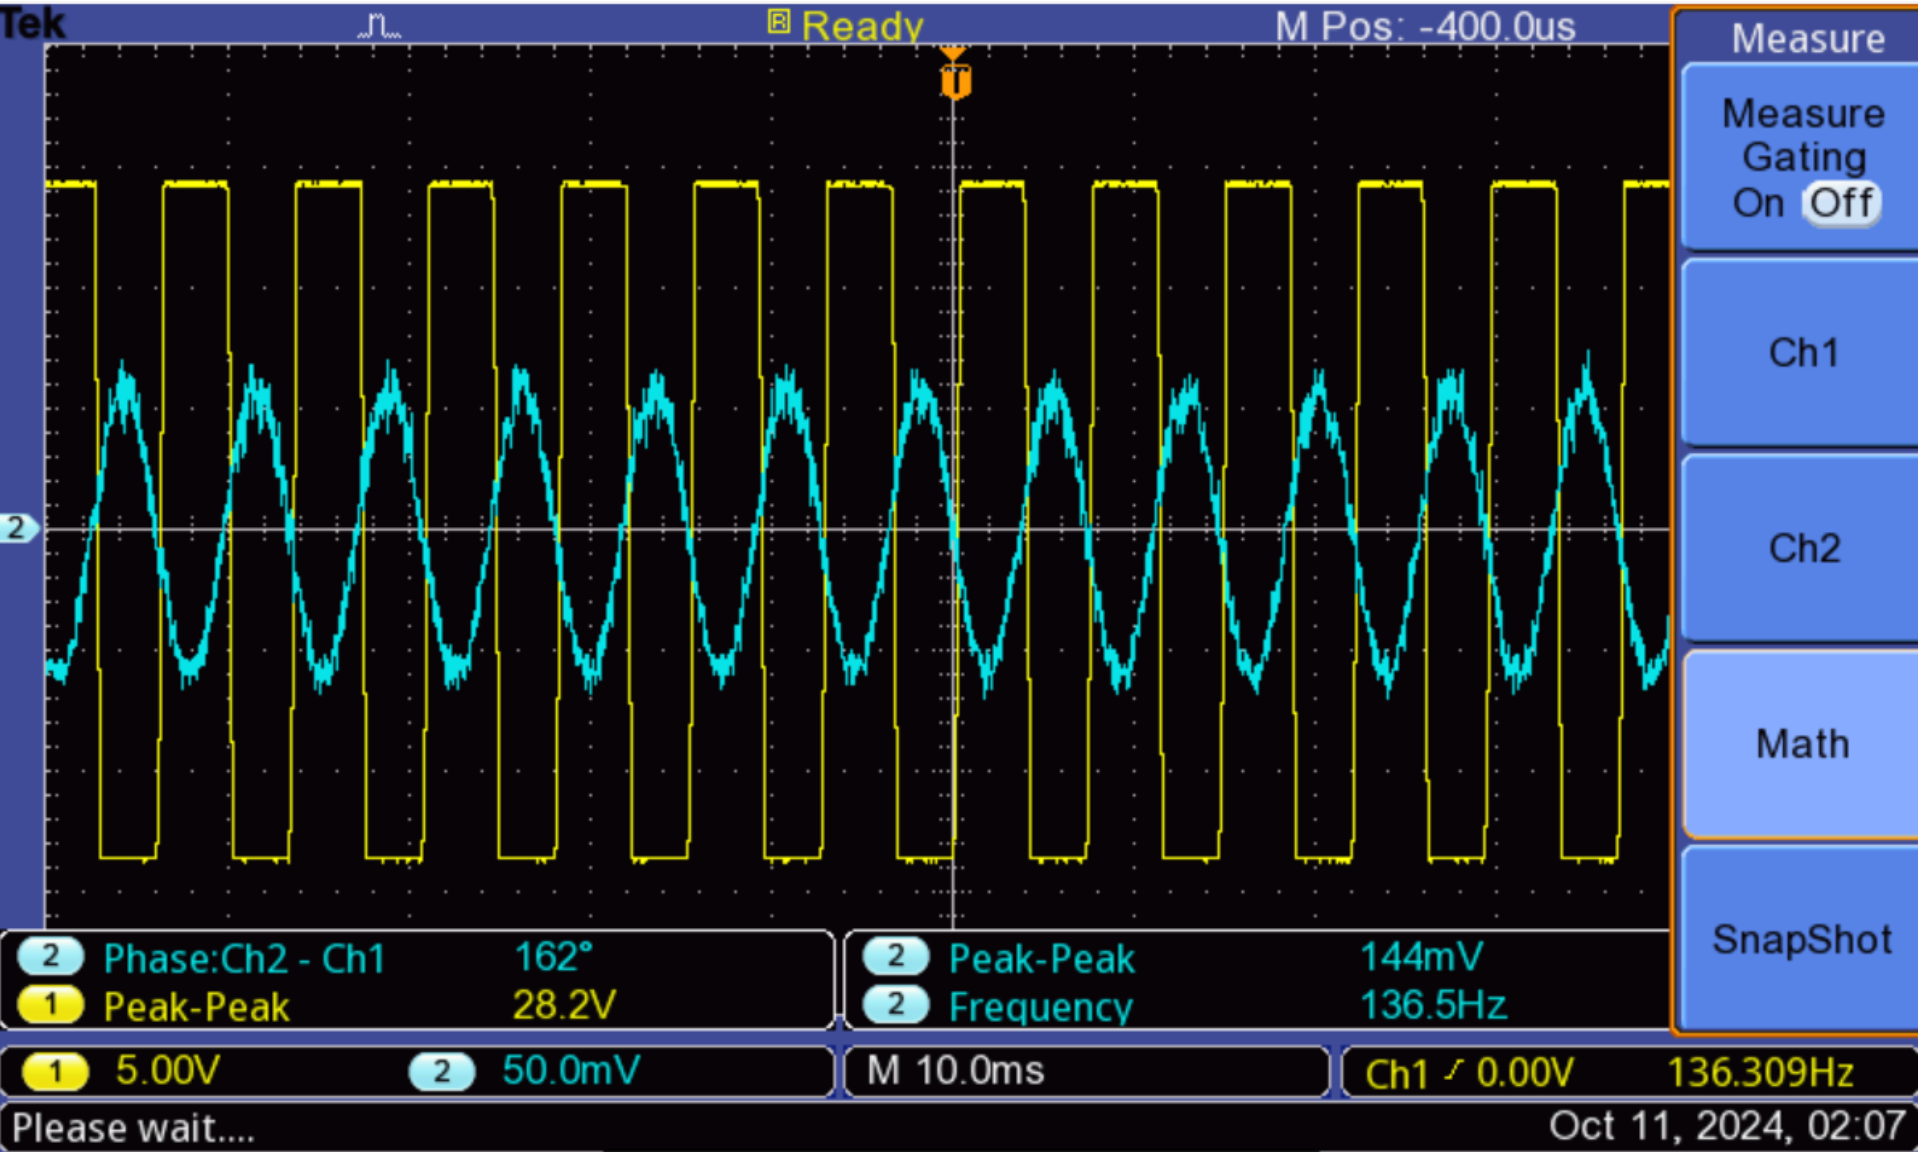
\includegraphics[width=0.8\textwidth]{img/Lab 7/1_2.png} % Update with actual image path
    \caption{}
\end{figure}

\begin{figure}[H]
    \centering
    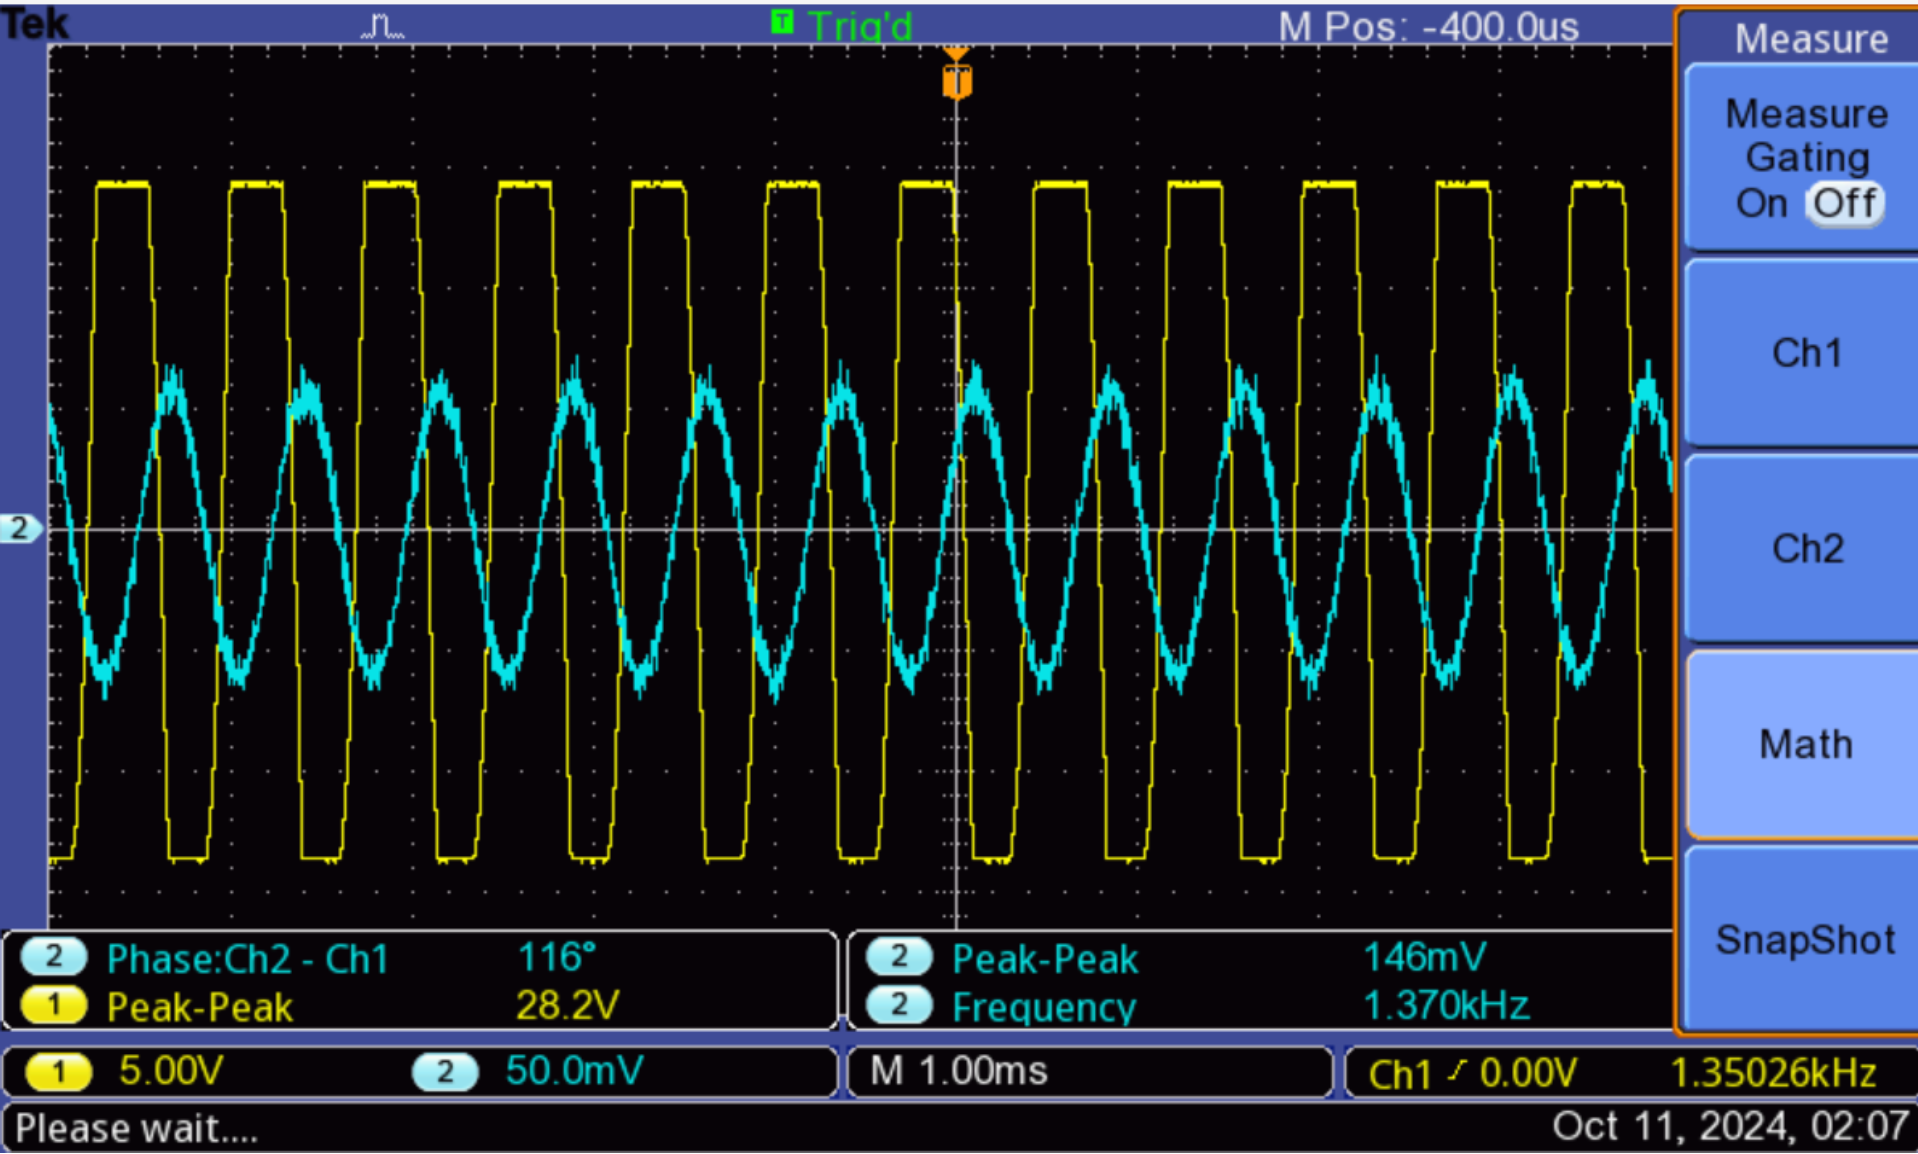
\includegraphics[width=0.8\textwidth]{img/Lab 7/1_3.png} % Update with actual image path
    \caption{}
\end{figure}

\begin{figure}[H]
    \centering
    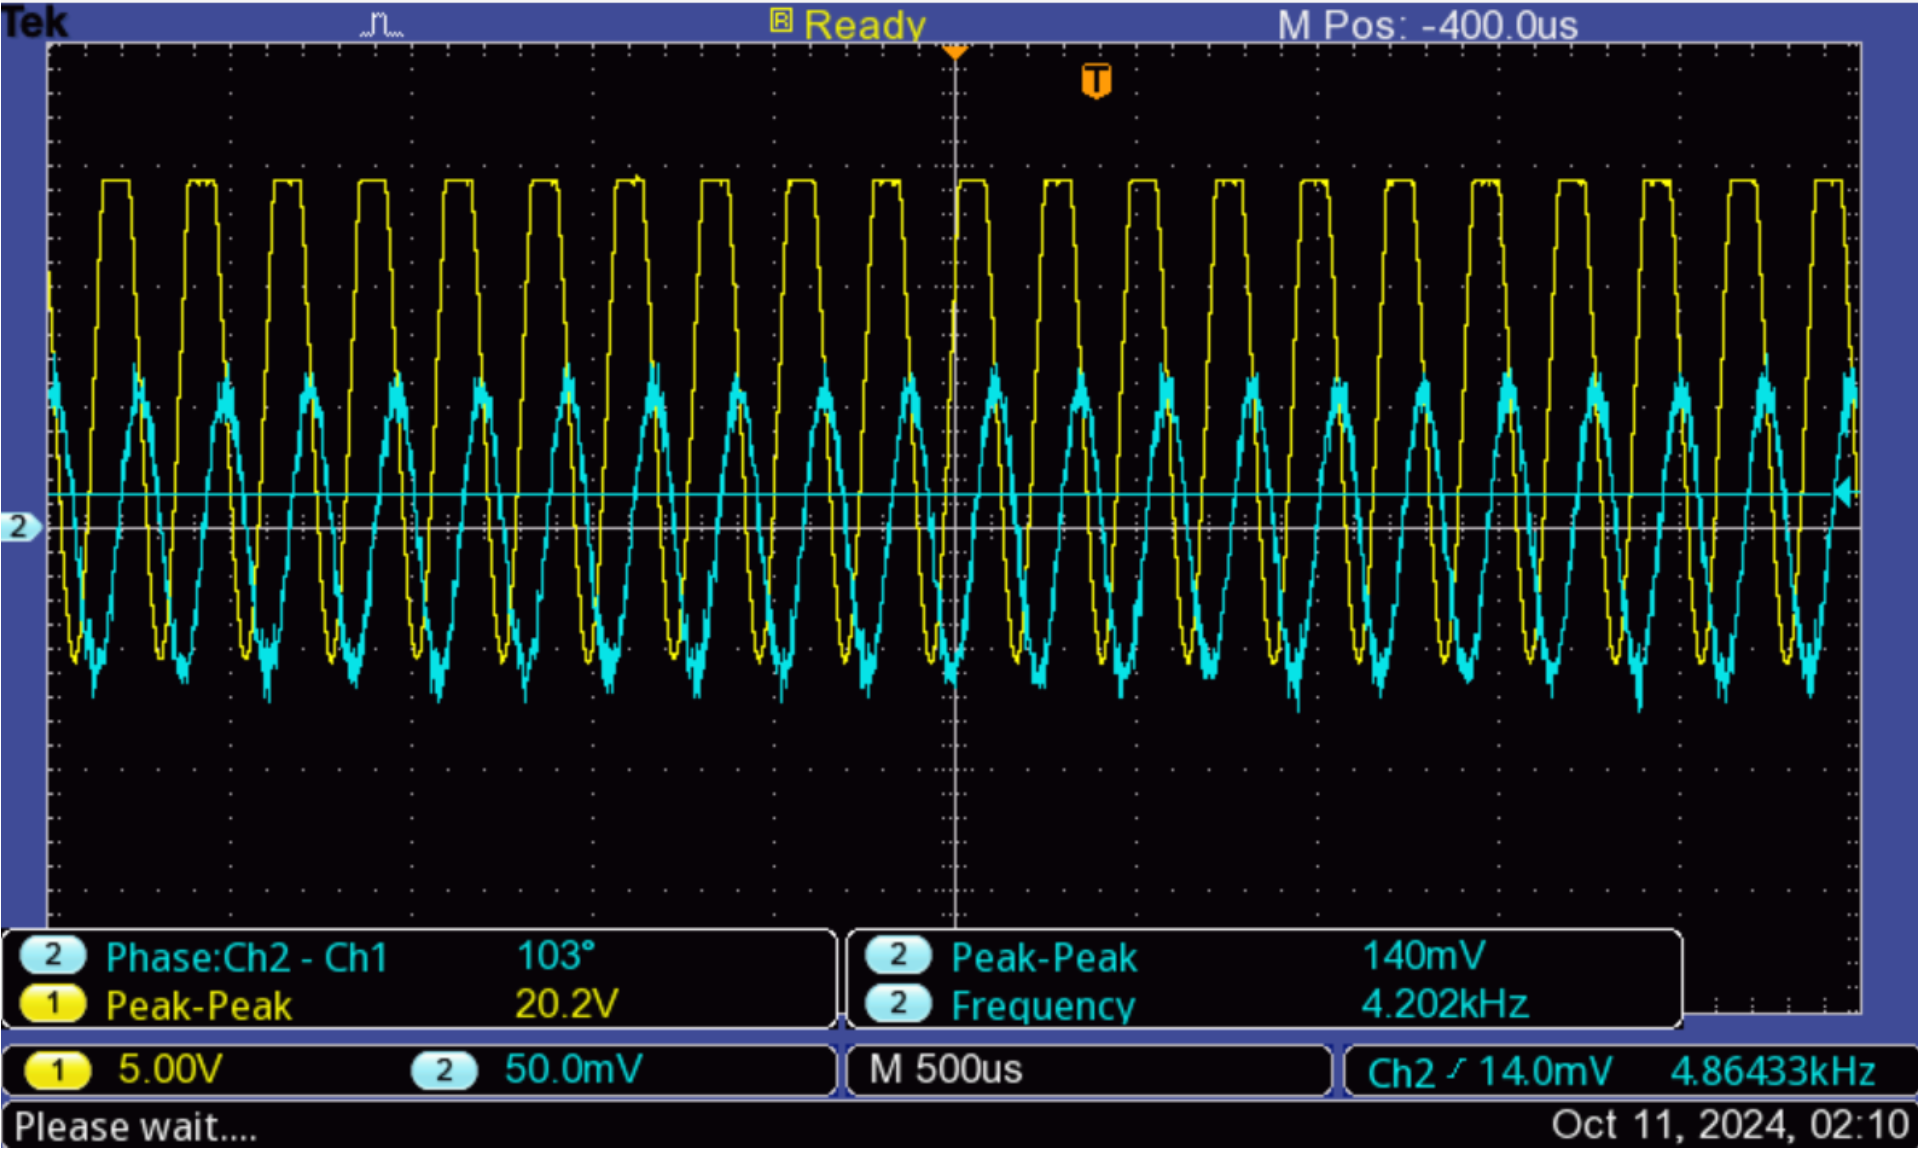
\includegraphics[width=0.8\textwidth]{img/Lab 7/1_4.png} % Update with actual image path
    \caption{}
\end{figure}

\begin{figure}[H]
    \centering
    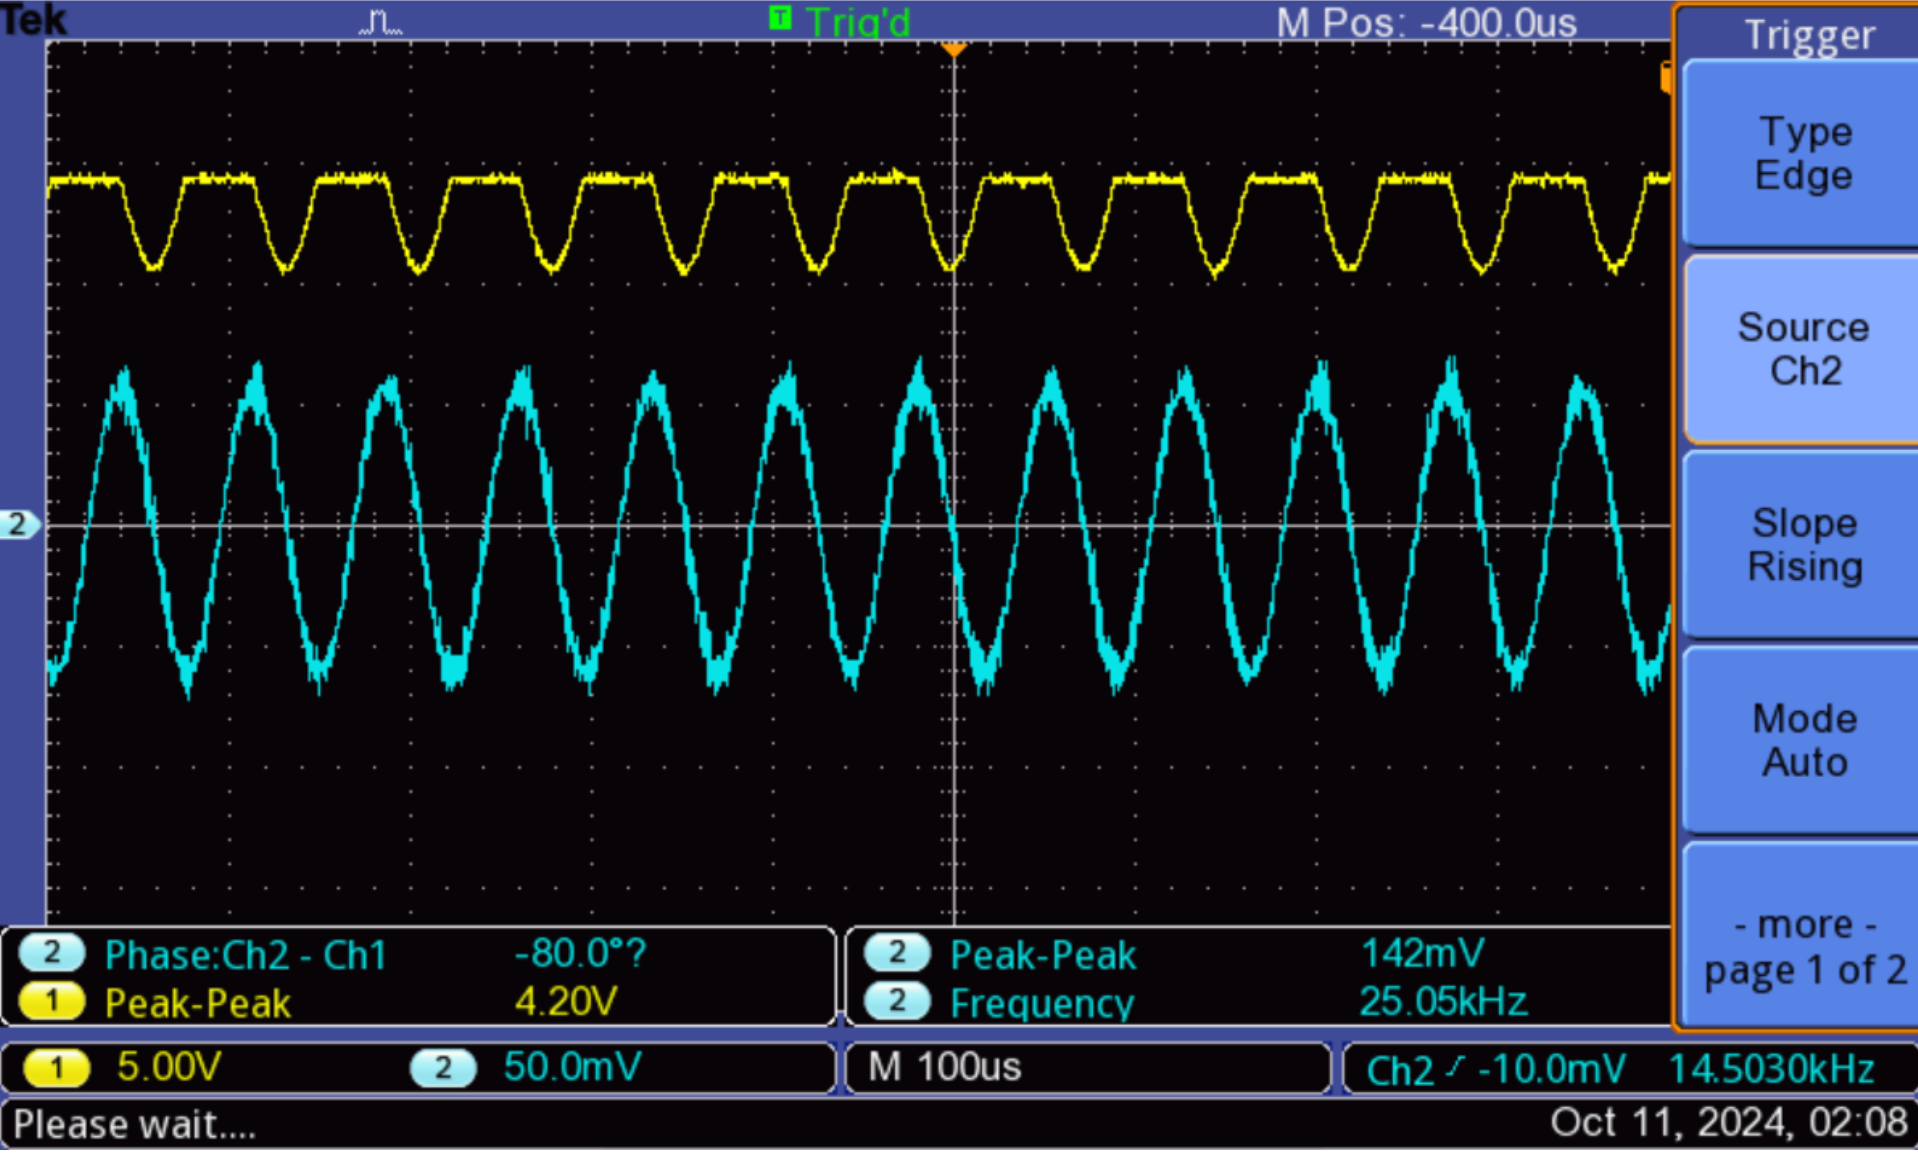
\includegraphics[width=0.8\textwidth]{img/Lab 7/1_5.png} % Update with actual image path
    \caption{}
\end{figure}

Our op-amp does not continue to compare throughout all frequencies and appears to stop
comparing at a frequency of \( 3.2 \, \text{kHz} \), the waveform for which is shown below.

\begin{figure}[H]
    \centering
    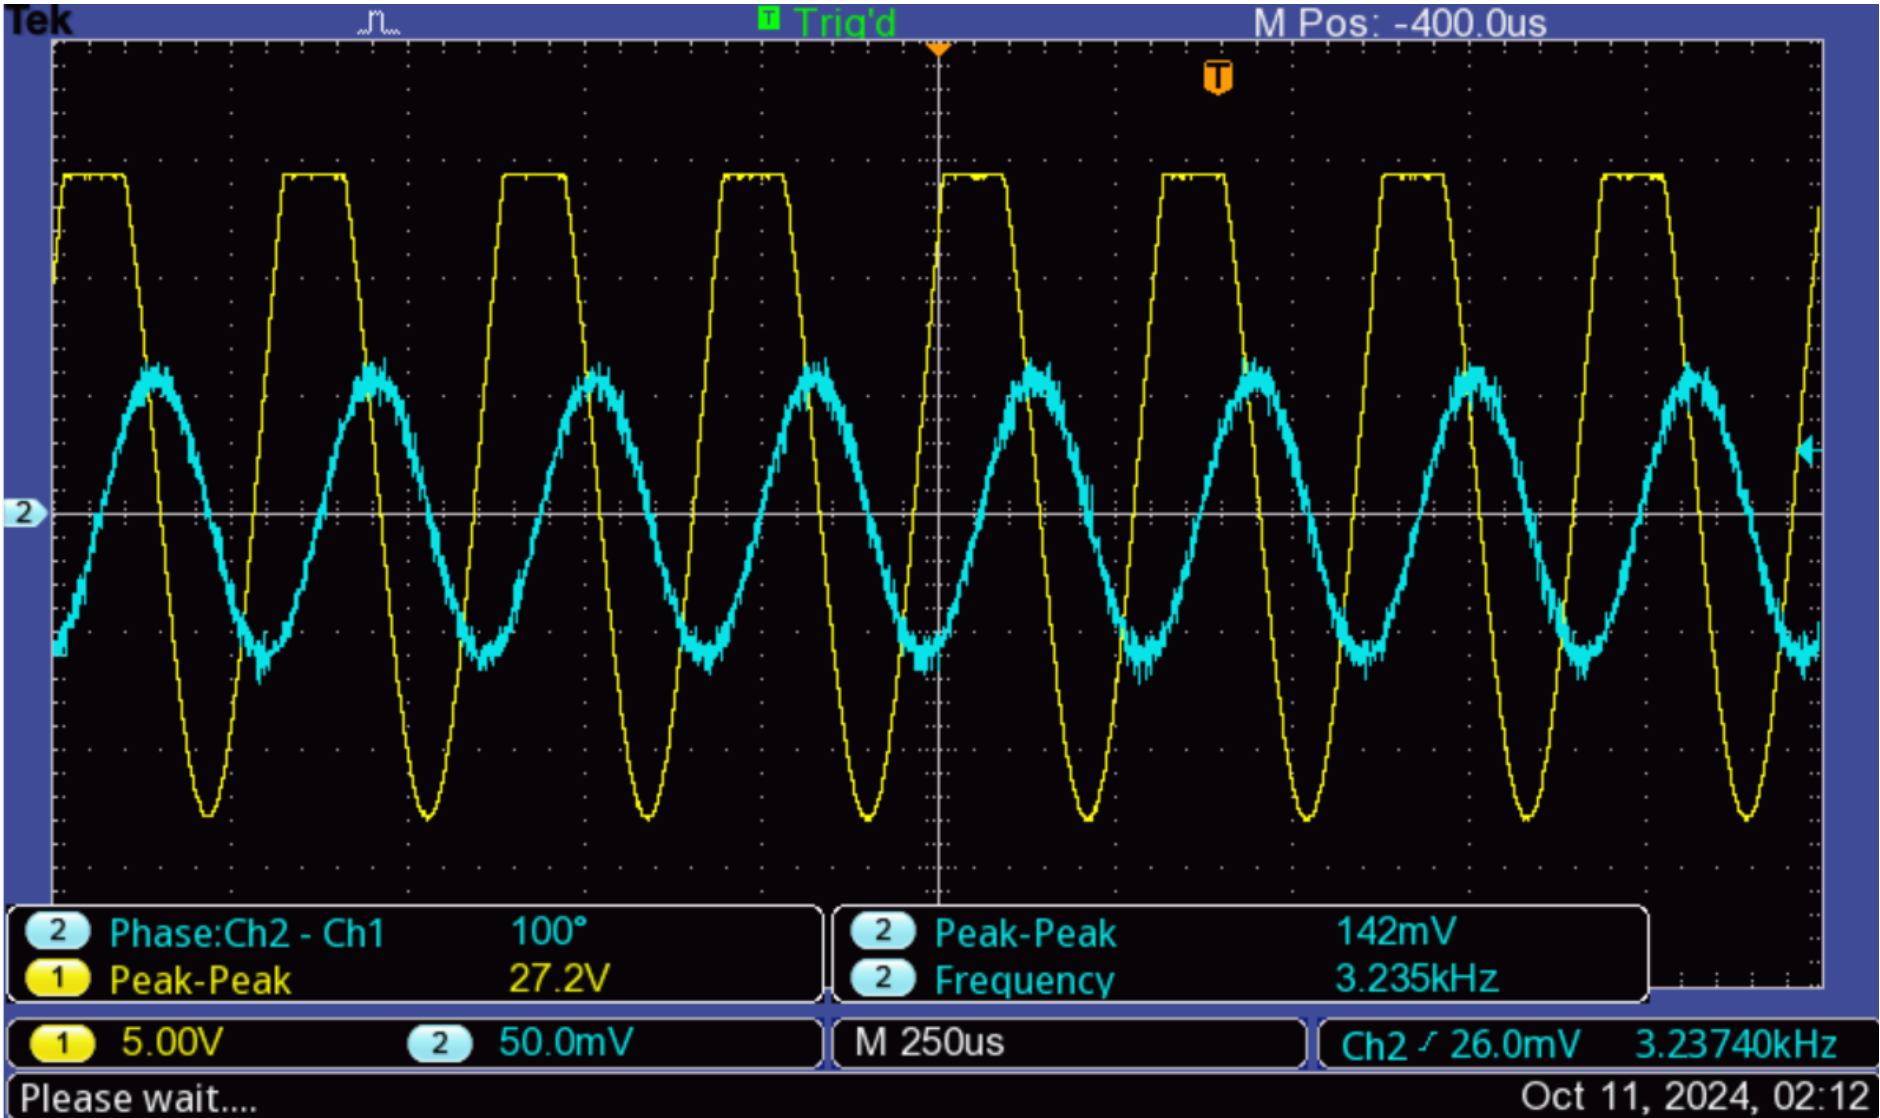
\includegraphics[width=0.8\textwidth]{img/Lab 7/1_6.png} % Update with actual image path
    \caption{Waveform at \( 3.2 \, \text{kHz} \)}
\end{figure}

"Comparating" refers to the op-amp's attempt to output a voltage very close to either the 
positive rail, \( V_{CC} \), or the negative rail, \( V_{EE} \), depending on 
whether \( V_{\text{in}} \) is less than or greater than the reference voltages \( V_{CC} \) 
or \( V_{EE} \). This behavior is due to its significant open-loop gain. At a certain 
frequency, \( V_{\text{out}} \) decreased, making the gain smaller and more difficult to maintain.
\\ \\
At a certain frequency, \( V_{\text{out}} \) decreased making the gain smaller making it more difficult to
compare changing voltages.

\subsection*{Question 2}
Build the amplifier in Fig. 3, measuring gain as \( -R_f/R_{in} \) with a ratio of 100.


\begin{table}[H]
    \centering
    \caption{Gain measurements for ratio of 10}
    \begin{tabular}{|c|c|c|}
    \hline
    \text{Frequency (Hz)} & \( V_{in} \) (mV) & \( V_{out} \) (mV) \\
    \hline
    100 & 328 & 2880 \\
    1k  & 328 & 2880 \\
    10k & 328 & 2880 \\
    100k & 328 & 3240 \\
    \hline
    \end{tabular}
\end{table}
\\ \\

\begin{table}[H]
\centering
\caption{Gain measurements for ratio of 100}
\begin{tabular}{|c|c|c|}
\hline
\text{Frequency (Hz)} & \( V_{in} \) (mV) & \( V_{out} \) (V) \\
\hline
100 & 304 & 25.8 \\
1k  & 304 & 25.8 \\
10k & 312 & 25.2 \\
40k & 312 & 25.2 \\
100k & 320 & 25.8 \\
\hline
\end{tabular}
\end{table}

\begin{figure}[H]
    \centering
    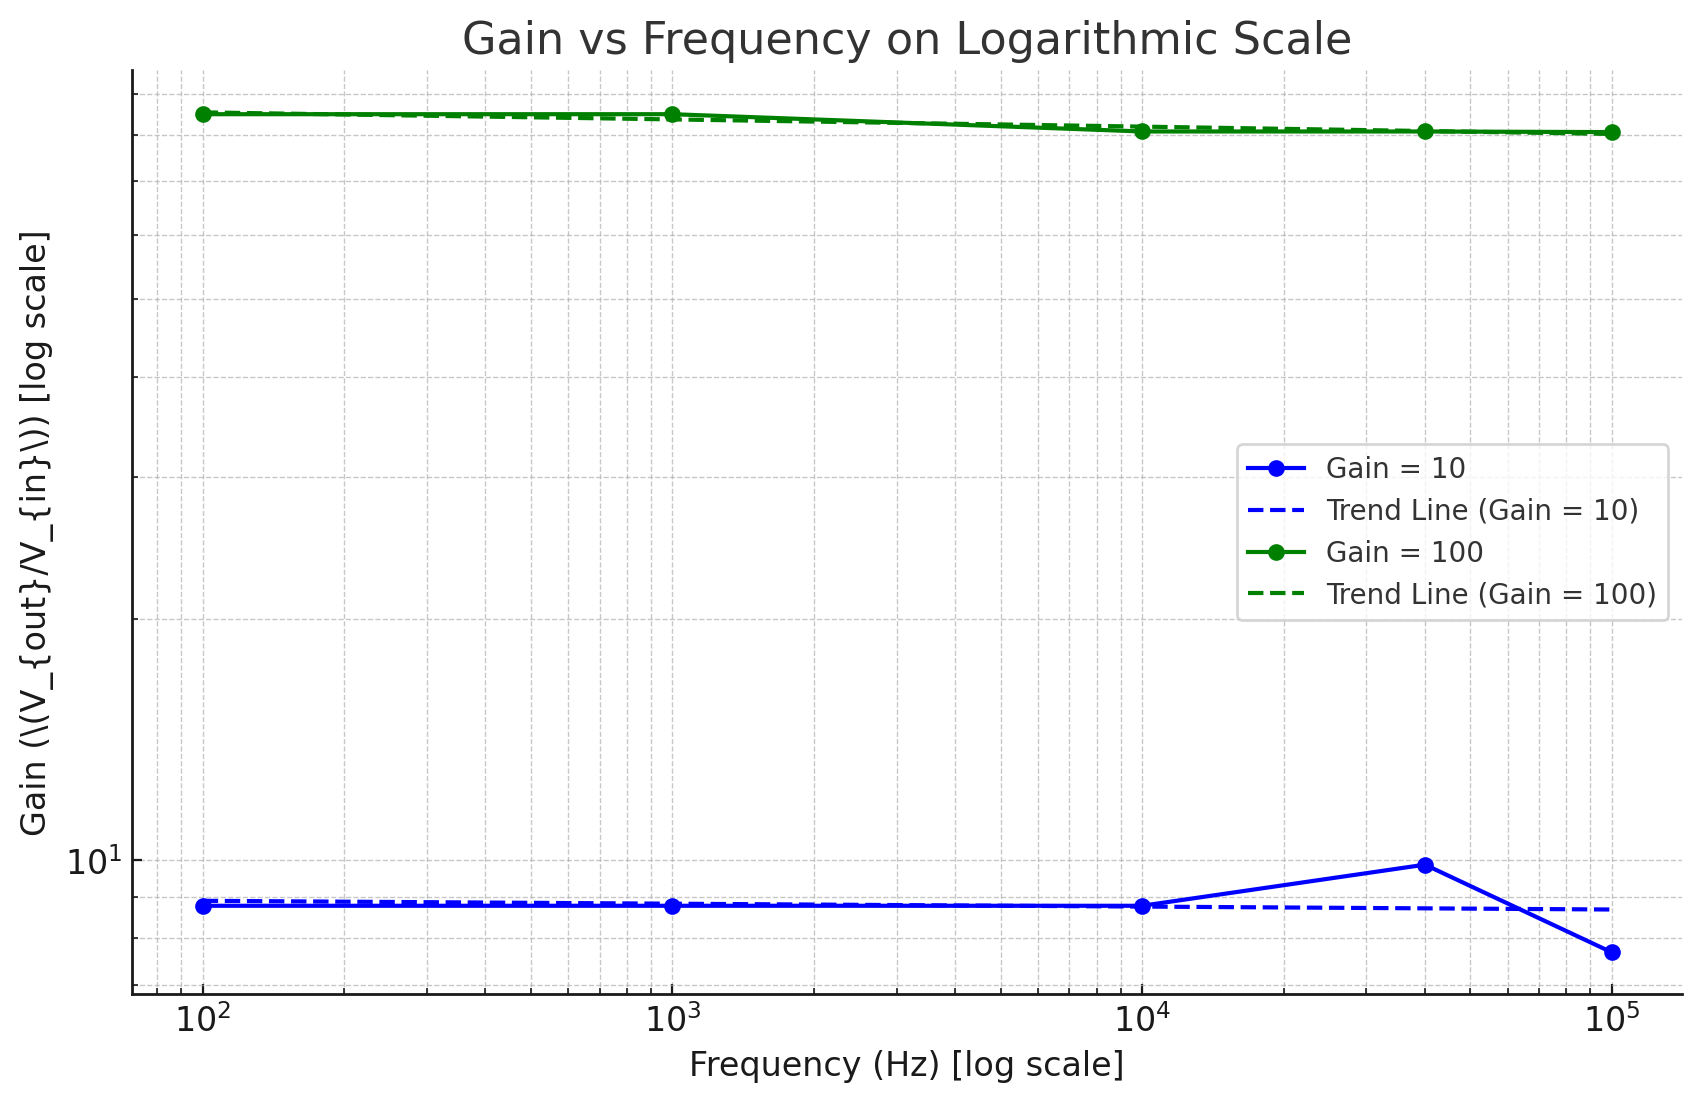
\includegraphics[width=0.8\textwidth]{img/Lab 7/2_2.png} % Update with actual image path
    \caption{Gain vs. Frequency on Logarithmic Scale for Gain = 10 and Gain = 100 with Trend Lines. The plot illustrates the relationship between the frequency of the input signal and the gain of the amplifier, showing a decrease in gain at higher frequencies for both configurations.}
\end{figure}

The plot shows how the gain behaves across a range of frequencies for two different gain 
settings: 10 and 100.

\begin{itemize}
    \item \textbf{Gain = 10:} The gain remains relatively stable across 
    the lower frequencies but shows a noticeable decline as the frequency 
    approaches 100 kHz. This behavior indicates that the amplifier can maintain 
    its gain effectively up to a certain frequency, after which it starts to 
    lose efficiency, possibly due to limitations in the op-amp's open-loop gain or bandwidth.
    \item \textbf{Gain = 100:} Similar to the Gain = 10 scenario, the gain starts high and 
    remains fairly consistent at lower frequencies but experiences a drop as the frequency 
    increases. The gain decreases more sharply compared to the Gain = 10 setting, indicating 
    that higher gain configurations are more susceptible to frequency-related losses.
\end{itemize}

The trend lines (dashed) demonstrate the overall decreasing trend of gain 
with increasing frequency, which is typical for amplifiers as they approach 
their frequency limits or bandwidth constraints. This drop in gain at higher 
frequencies is due to the op-amp's inability to respond quickly enough to 
the rapid changes in the input signal, leading to reduced amplification.

\subsection*{Question 3}
Using the two fundamental op-amp rules:

\begin{enumerate}
    \item The output adjusts itself to make the voltage difference between the inverting and non-inverting inputs as close to zero as possible.
    \item The inputs draw no current.
\end{enumerate}

We can understand how the gain of the inverting amplifier is determined. Since 
no current flows into the inputs of the op-amp, the current through the feedback 
resistor \( R_f \) must equal the current through the input resistor \( R_{in} \). 
This creates a voltage difference that is directly proportional to the input 
voltage \( V_{\text{in}} \), scaled by the ratio \( R_f/R_{in} \).

The op-amp works to minimize the voltage difference between its inputs by 
adjusting the output voltage \( V_{\text{out}} \). As a result, the output 
voltage is given by the expression \( V_{\text{out}} = -\frac{R_f}{R_{in}} V_{\text{in}} \), 
which represents the gain of the inverting amplifier. Additionally, because there is 
no current through \( R_g \), the inverting input behaves like an extended virtual ground.

\subsection*{Question 4}
Using the summing amplifier configuration, we measured the output voltage \( V_{\text{out}} \) for different combinations of input voltages \( V_1 \) and \( V_2 \), and resistances \( R_1 \), \( R_2 \), and \( R_f \).

The output voltage \( V_{\text{out}} \) is given by:
\[
V_{\text{out}} = -\left(\frac{R_f}{R_1} V_1 + \frac{R_f}{R_2} V_2\right)
\]

\begin{figure}[H]
    \centering
    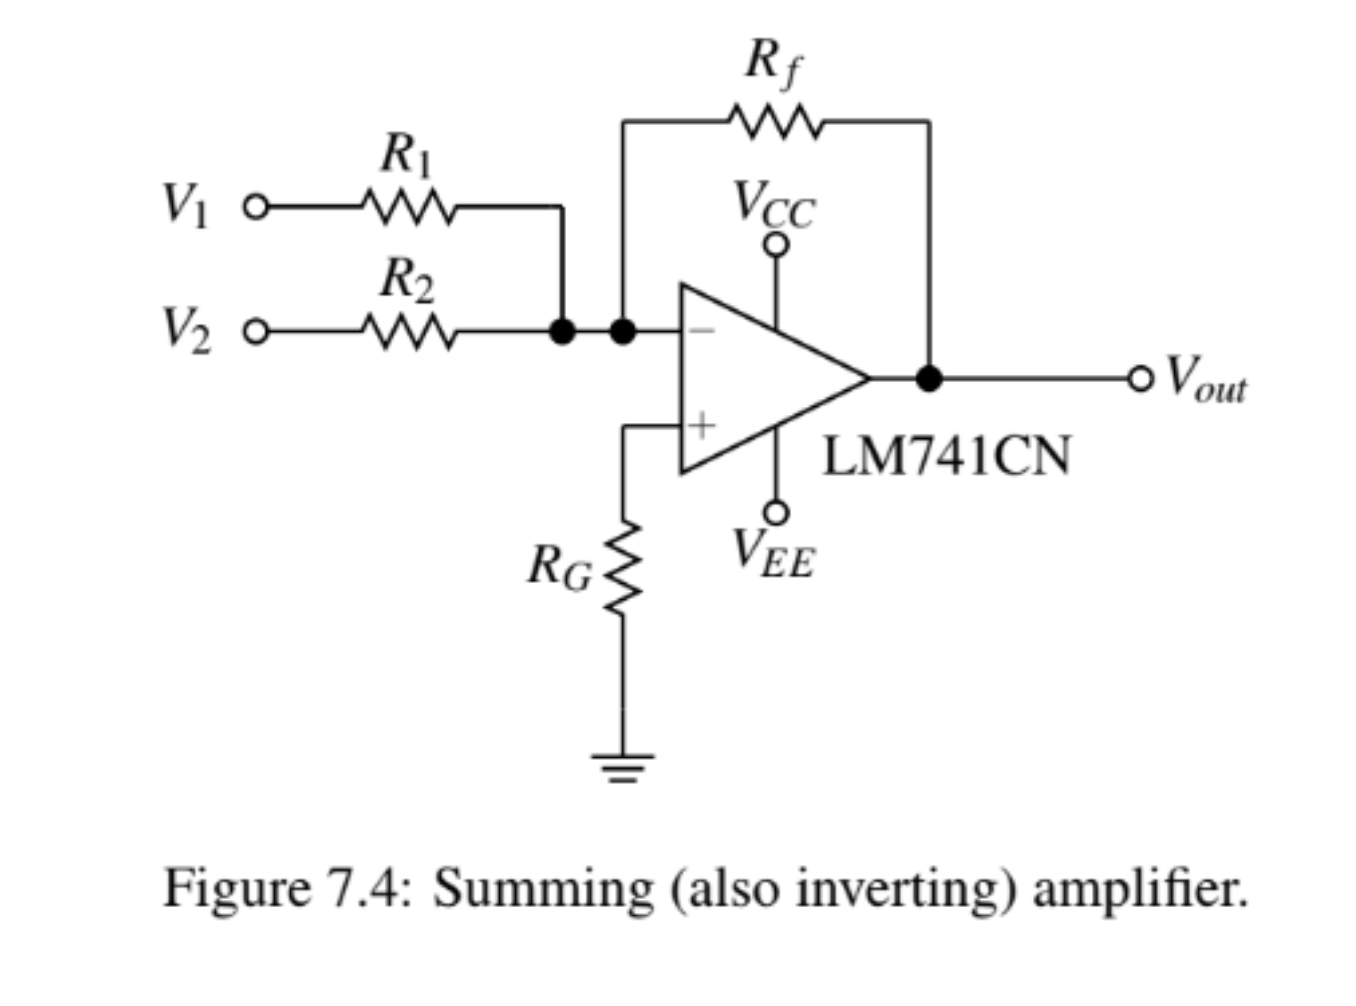
\includegraphics[width=0.8\textwidth]{img/Lab 7/4_1.png} % Update with actual image path
    \caption{}
\end{figure}

Below is the table of our measurements:

\begin{table}[H]
\centering
\caption{Summing Amplifier Measurements}
\begin{tabular}{|c|c|c|c|c|c|}
\hline
\textbf{\( V_1 \) (V)} & \textbf{\( V_2 \) (V)} & \textbf{\( R_1 \) (k\(\Omega\))} & \textbf{\( R_2 \) (k\(\Omega\))} & \textbf{\( R_f \) (k\(\Omega\))} & \textbf{\( V_{\text{out}} \) (V)} \\
\hline
2.5 & 2.5 & 1   & 1   & 1   & -0.48 \\
2.5 & 2.5 & 10  & 10  & 1   & -4.92 \\
5   & 5   & 10  & 10  & 10  & -9.9  \\
5   & 5   & 100 & 10  & 10  & -5.4  \\
5   & 5   & 10  & 10  & 1   & -0.99 \\
7.5 & 7.5 & 10  & 10  & 1   & -1.47 \\
\hline
\end{tabular}
\end{table}

We observed that whenever \( R_f \) was significantly larger than \( R_1 \) and \( R_2 \), \( V_{\text{out}} \)
became overloaded due to an excessive amplification factor. This caused the output to default to 
the breadboard's maximum voltage of approximately \( 15 \, \text{V} \).

\subsection*{Question 5}

We are now tasked with using the data collected from Question 4 to derive 
an equation for \( V_{\text{out}} \) as a function of \( V_1 \), \( V_2 \), \( R_1 \), \( R_2 \), and \( R_f \). 
Additionally, we need to generalize this formula for \( V_n \) and \( R_n \).

Since \( V_{\text{out}} \) is consistently negative, and we are working with an inverting 
amplifier, we can assume the gain is given by \( -\frac{R_f}{R_{\text{in}}} \). 
Given \( n \) values for \( R_{\text{in}} \), we can express a portion of \( V_{\text{out}} \) as:

\[
V_{\text{out}} = -\frac{R_f}{R_1} + \ldots + -\frac{R_f}{R_n}
\]

Since gain is dimensionless, but \( V_{\text{out}} \) is measured in 
volts, we multiply by the input voltages \( V_{\text{in}} \) to obtain:

\[
V_{\text{out}} = -\frac{R_f}{R_{\text{in}}} \times V_{\text{in}}
\]

By combining these concepts, we derive the general solution:

\[
V_{\text{out}} = -\frac{R_f}{R_1} V_1 + \ldots + -\frac{R_f}{R_n} V_n
\]

To match this to the summing (inverting) amplifier, the equation simplifies to:

\[
V_{\text{out}} = -\frac{R_f}{R_1} V_1 - \frac{R_f}{R_2} V_2
\]

Applying our data to this formula yields a calculated \( V_{\text{out}} \) that closely 
matches the measured \( V_{\text{out}} \), with an error of approximately 1.8\%.

As noted in Question 4, if the calculated \( V_{\text{out}} \) exceeds the 
limits of \( V_{EE} \) or \( V_{CC} \), the output will become overloaded 
and default to the voltage of the positive (\(+\)) or negative (\(-\)) rail.


\subsection*{Bonus Question}

Using the summing amplifier configuration from Questions 4 and 5, 
with \( R_1 = R_2 = R_f \), we applied sine waves to both inputs. 
Initially, we set both input frequencies to \( 10 \, \text{kHz} \), 
and then varied them to observe the interaction between the waves.

When the frequencies were close to each other, the resulting 
output appeared as a single sine wave, demonstrating constructive 
interference. However, as the frequencies diverged, the output 
displayed a superposition of waves. This resulted in distinct wave 
packets, where each packet contained segments of individual sine 
waves corresponding to the different input frequencies.

\begin{figure}[H]
    \centering
    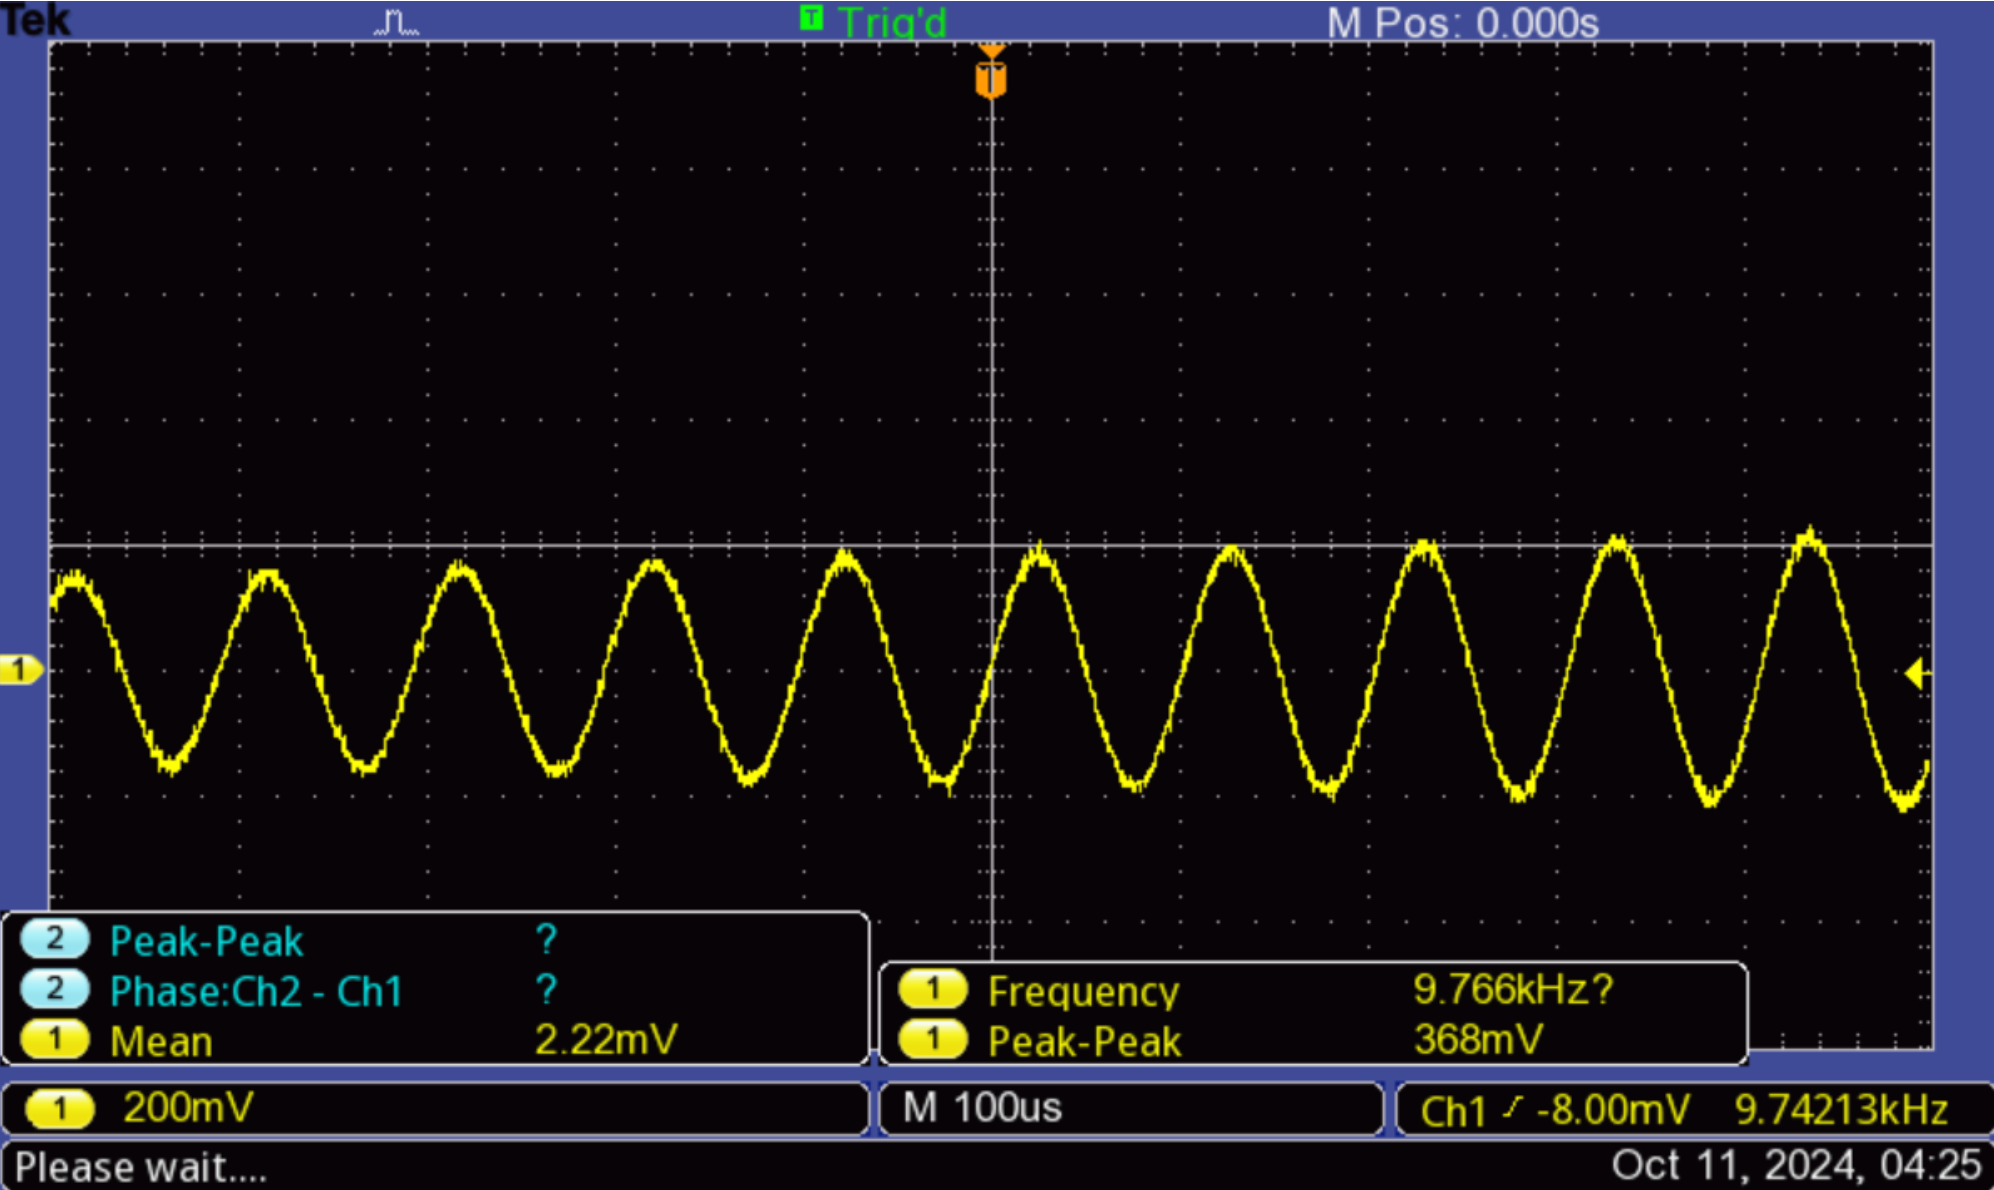
\includegraphics[width=0.8\textwidth]{img/Lab 7/b_1.png} 
    \caption{f1 = f2 = 10kHz}
\end{figure}

\begin{figure}[H]
    \centering
    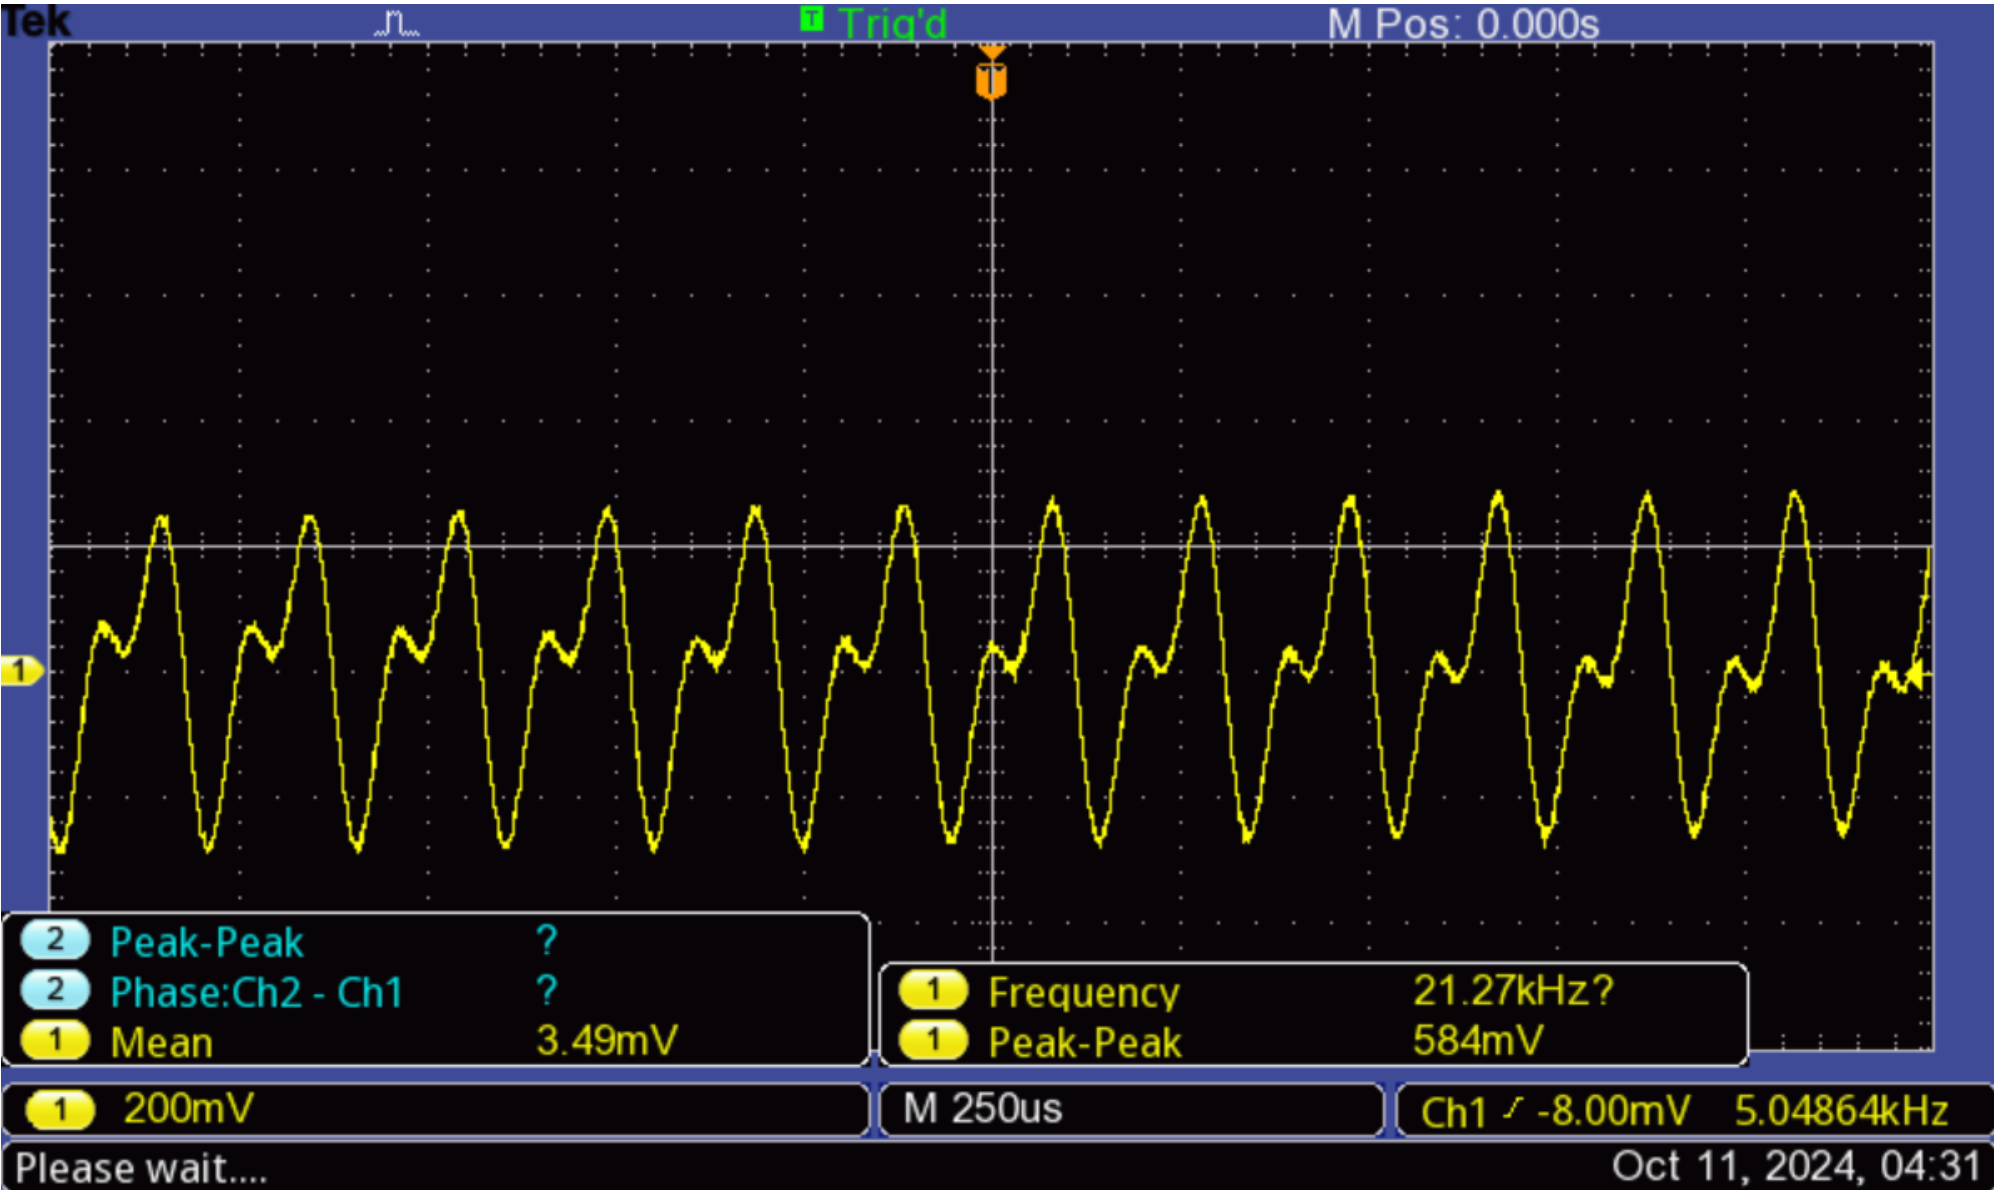
\includegraphics[width=0.8\textwidth]{img/Lab 7/b_2.png}
    \caption{f1 = 10kHz f2 = 12kHz}
\end{figure}

\begin{figure}[H]
    \centering
    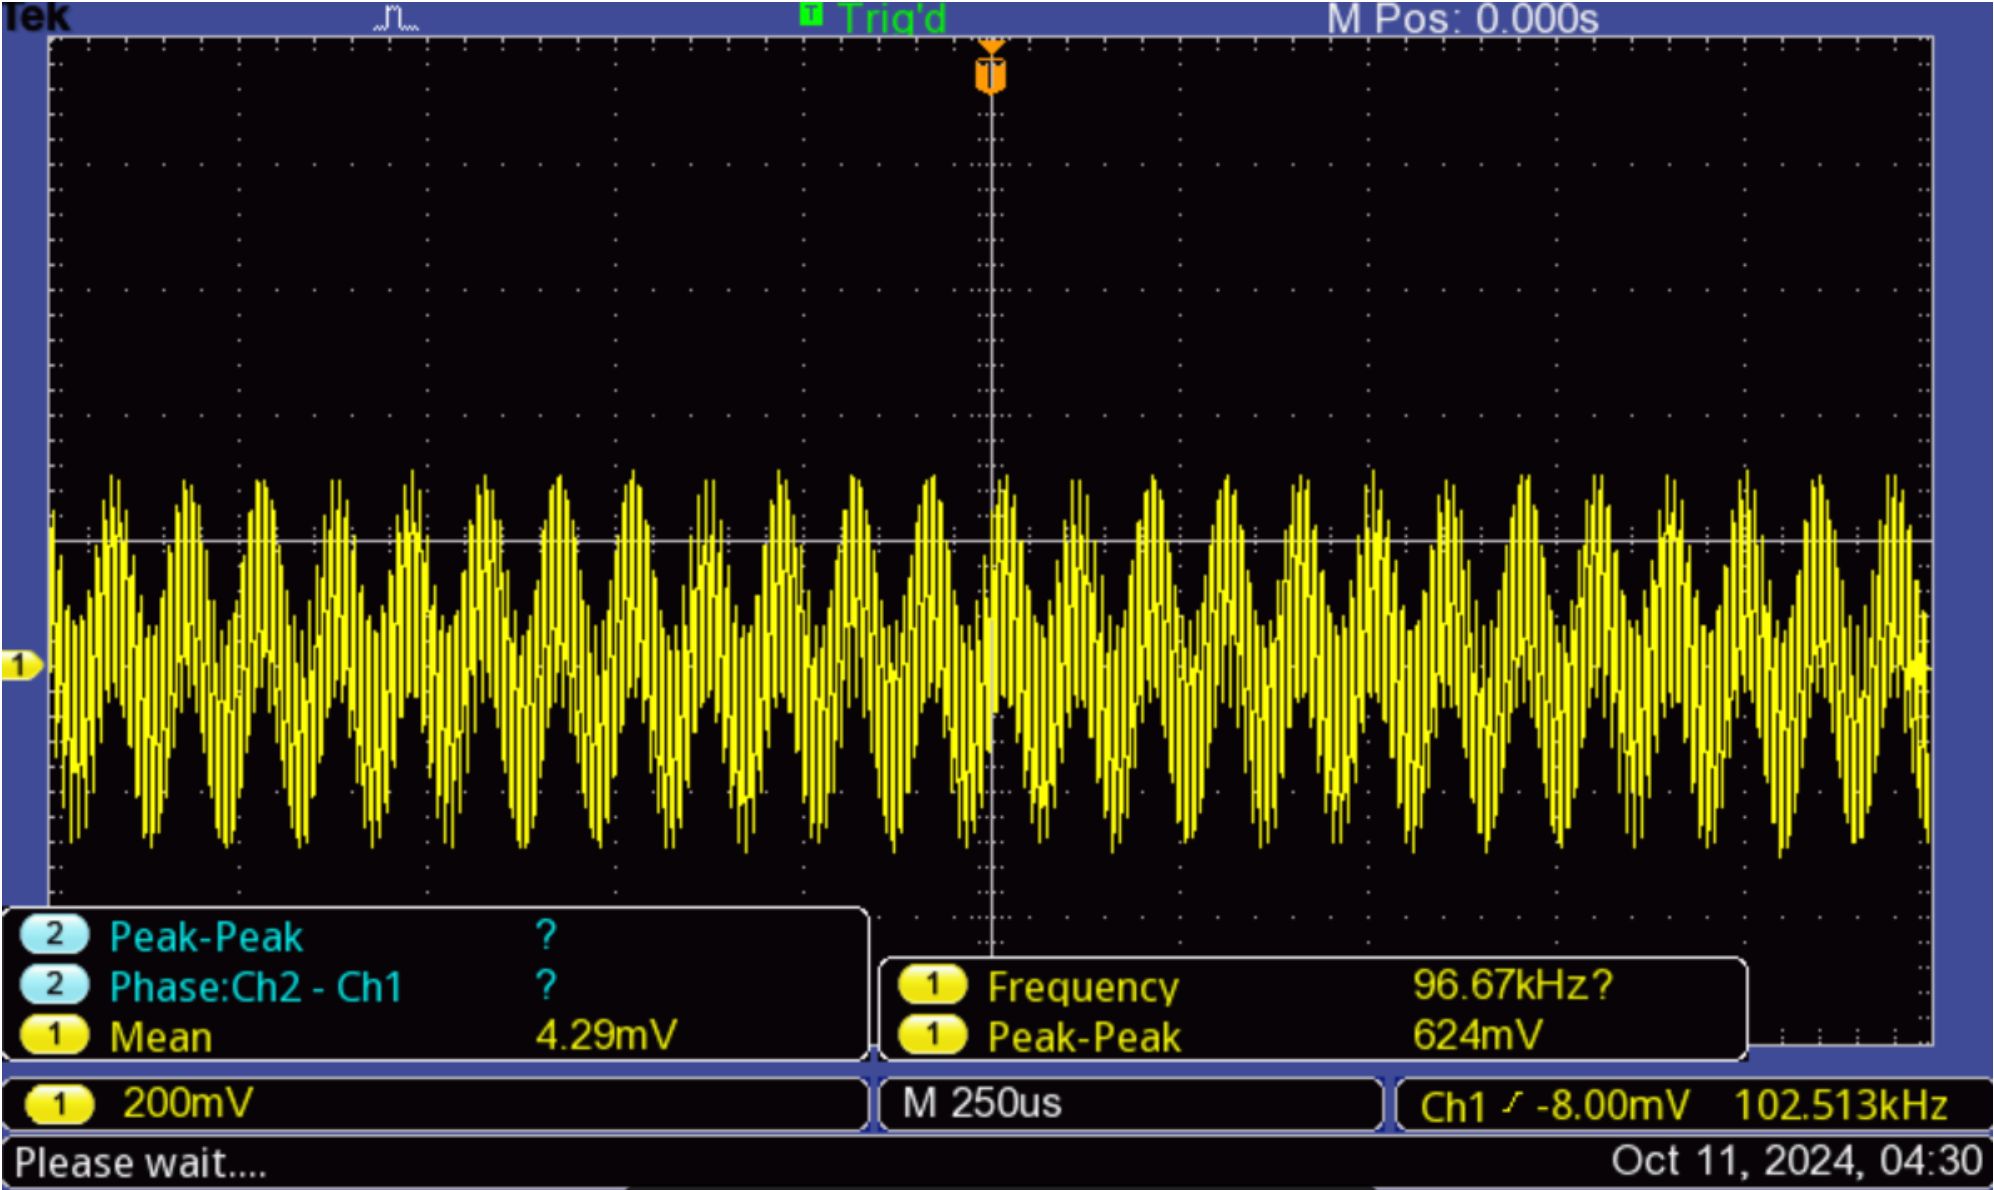
\includegraphics[width=0.8\textwidth]{img/Lab 7/b_3.png} 
    \caption{f1 = 10kHz f2 = 100kHz}
\end{figure}


Observations include: \\ 
- \( f_1 = f_2 = 10kHz \): Waves perfectly superimpose. \\ 
- \( f_1 = 10kHz, f_2 = 12kHz \): Slight divergence observed.\\
- \( f_1 = 10kHz, f_2 = 100kHz \): Distinct superposition patterns. \\





\section*{Lab 8: Operational Amplifiers II}

\subsection*{Introduction}
In this lab, we explored three different operational amplifier (op-amp) 
circuits: an integrator, a comparator without feedback, and a comparator 
with feedback (Schmitt trigger). The objective was to build, observe, and 
analyze the behavior of these circuits.

\subsection*{Question 1}
\textbf{Objective:} Build an op-amp integrator circuit using a 
capacitor \( C_f \) and input resistance \( R_{\text{in}} \), 
and determine the frequency range over which the circuit produces 
the integral of \( V_{\text{in}} \).

\textbf{Procedure:} \\ 
- A square wave input was applied to the circuit. \\ 
- The output waveforms were observed at various frequencies using an oscilloscope. \\ 
\\ 

\begin{figure}[H]
    \centering
    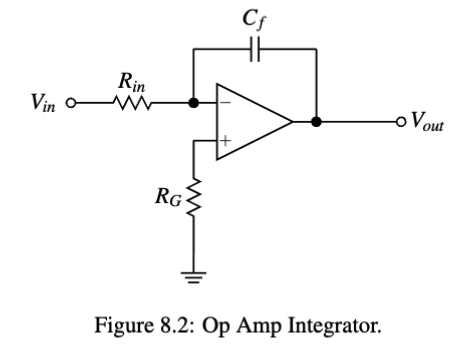
\includegraphics[width=0.8\textwidth]{img/Lab 8/1_1.png} % Replace with actual image
    \caption{Output waveforms at various frequencies}
\end{figure}

\textbf{Observation:}
At lower frequencies, the circuit effectively integrates the input, 
resulting in a triangular waveform. As the frequency increases, the 
integration behavior diminishes, producing a distorted output.
\\ \\ 

Below are the output waveforms displaying the frequency range in practice in the follow-
ing order; 900Hz, 9.8kHz, 121kHz, 422kHz

\begin{figure}[H]
    \centering
    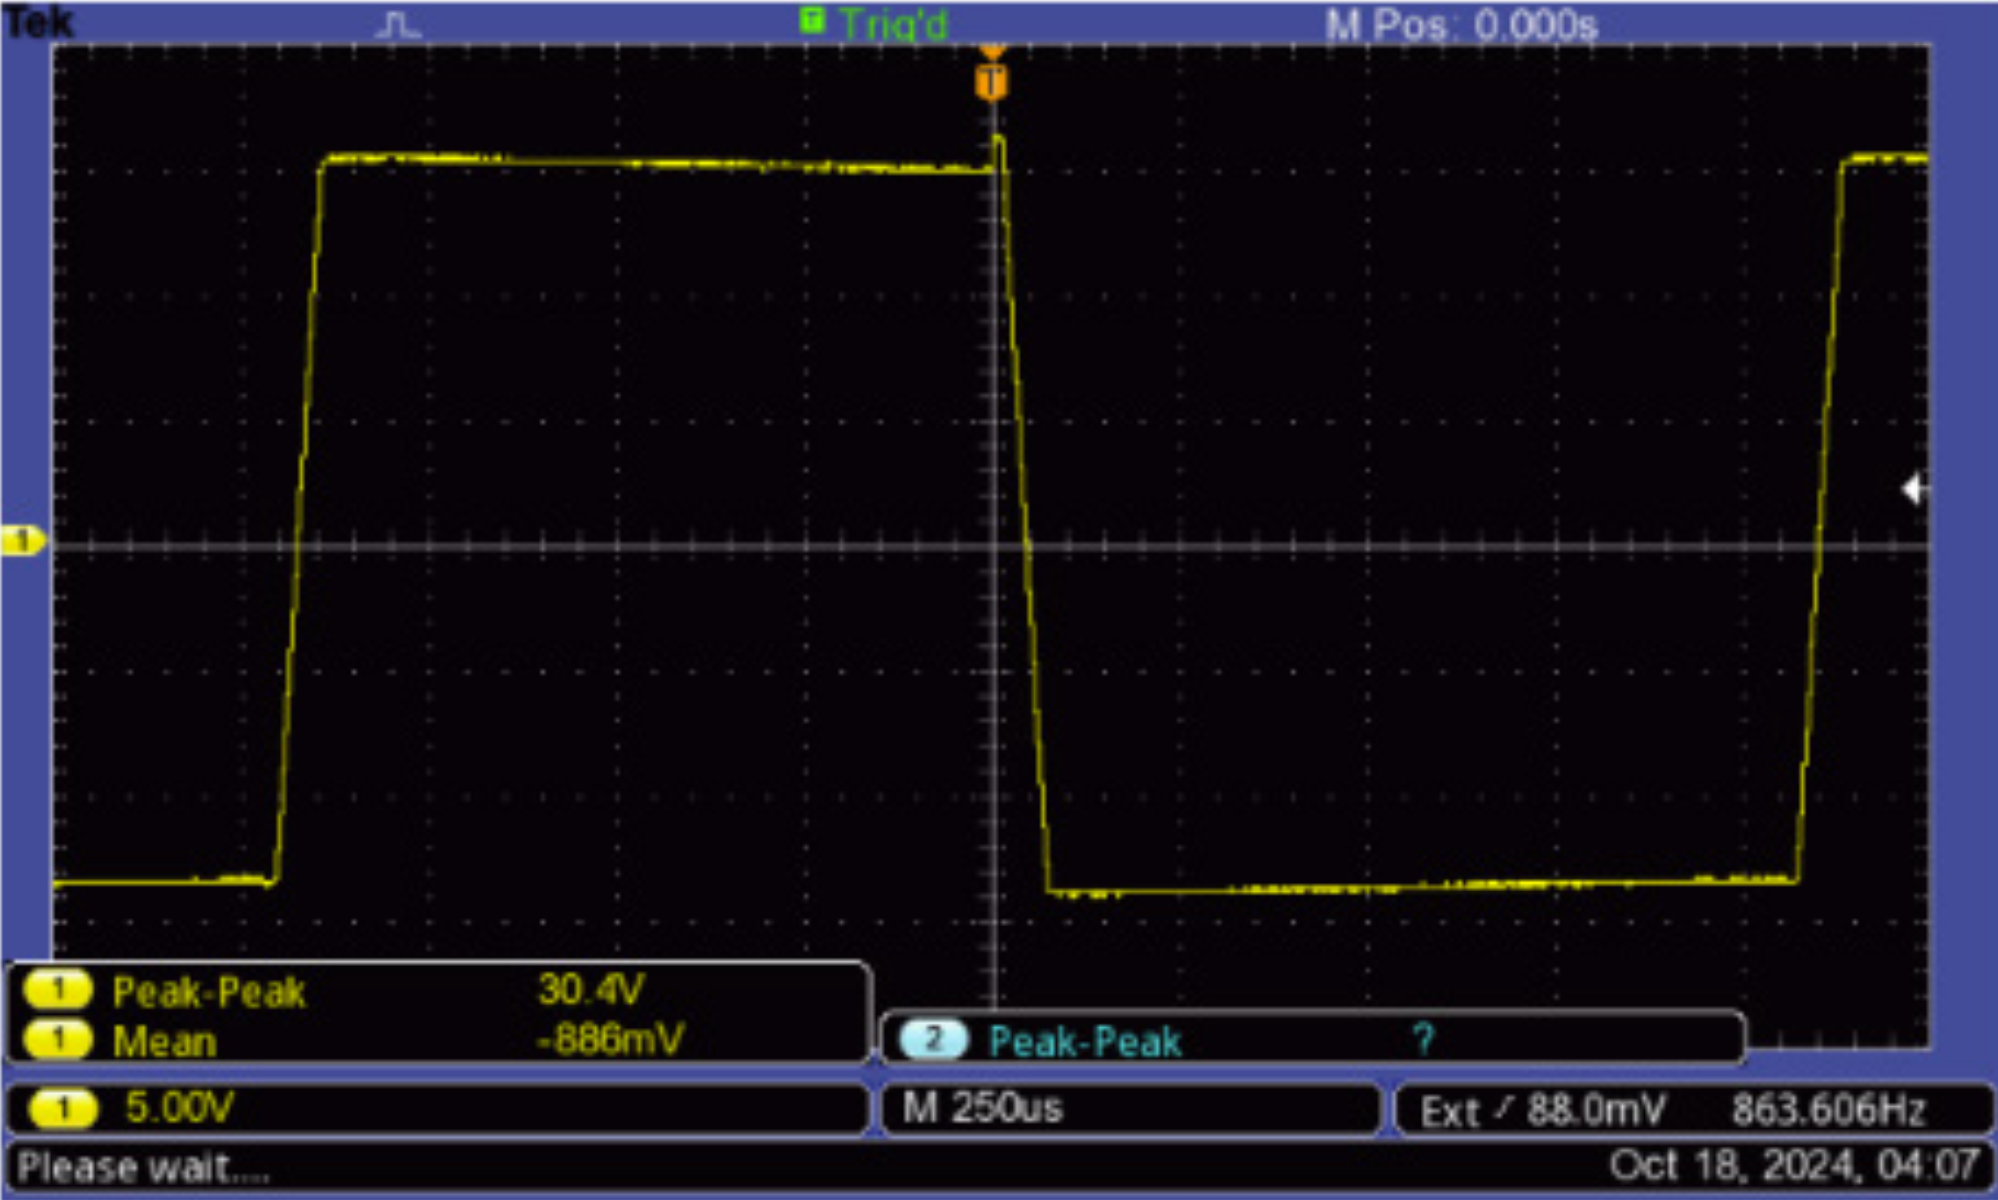
\includegraphics[width=0.8\textwidth]{img/Lab 8/1_2.png} % Replace with actual image
    \caption{}
\end{figure}

\begin{figure}[H]
    \centering
    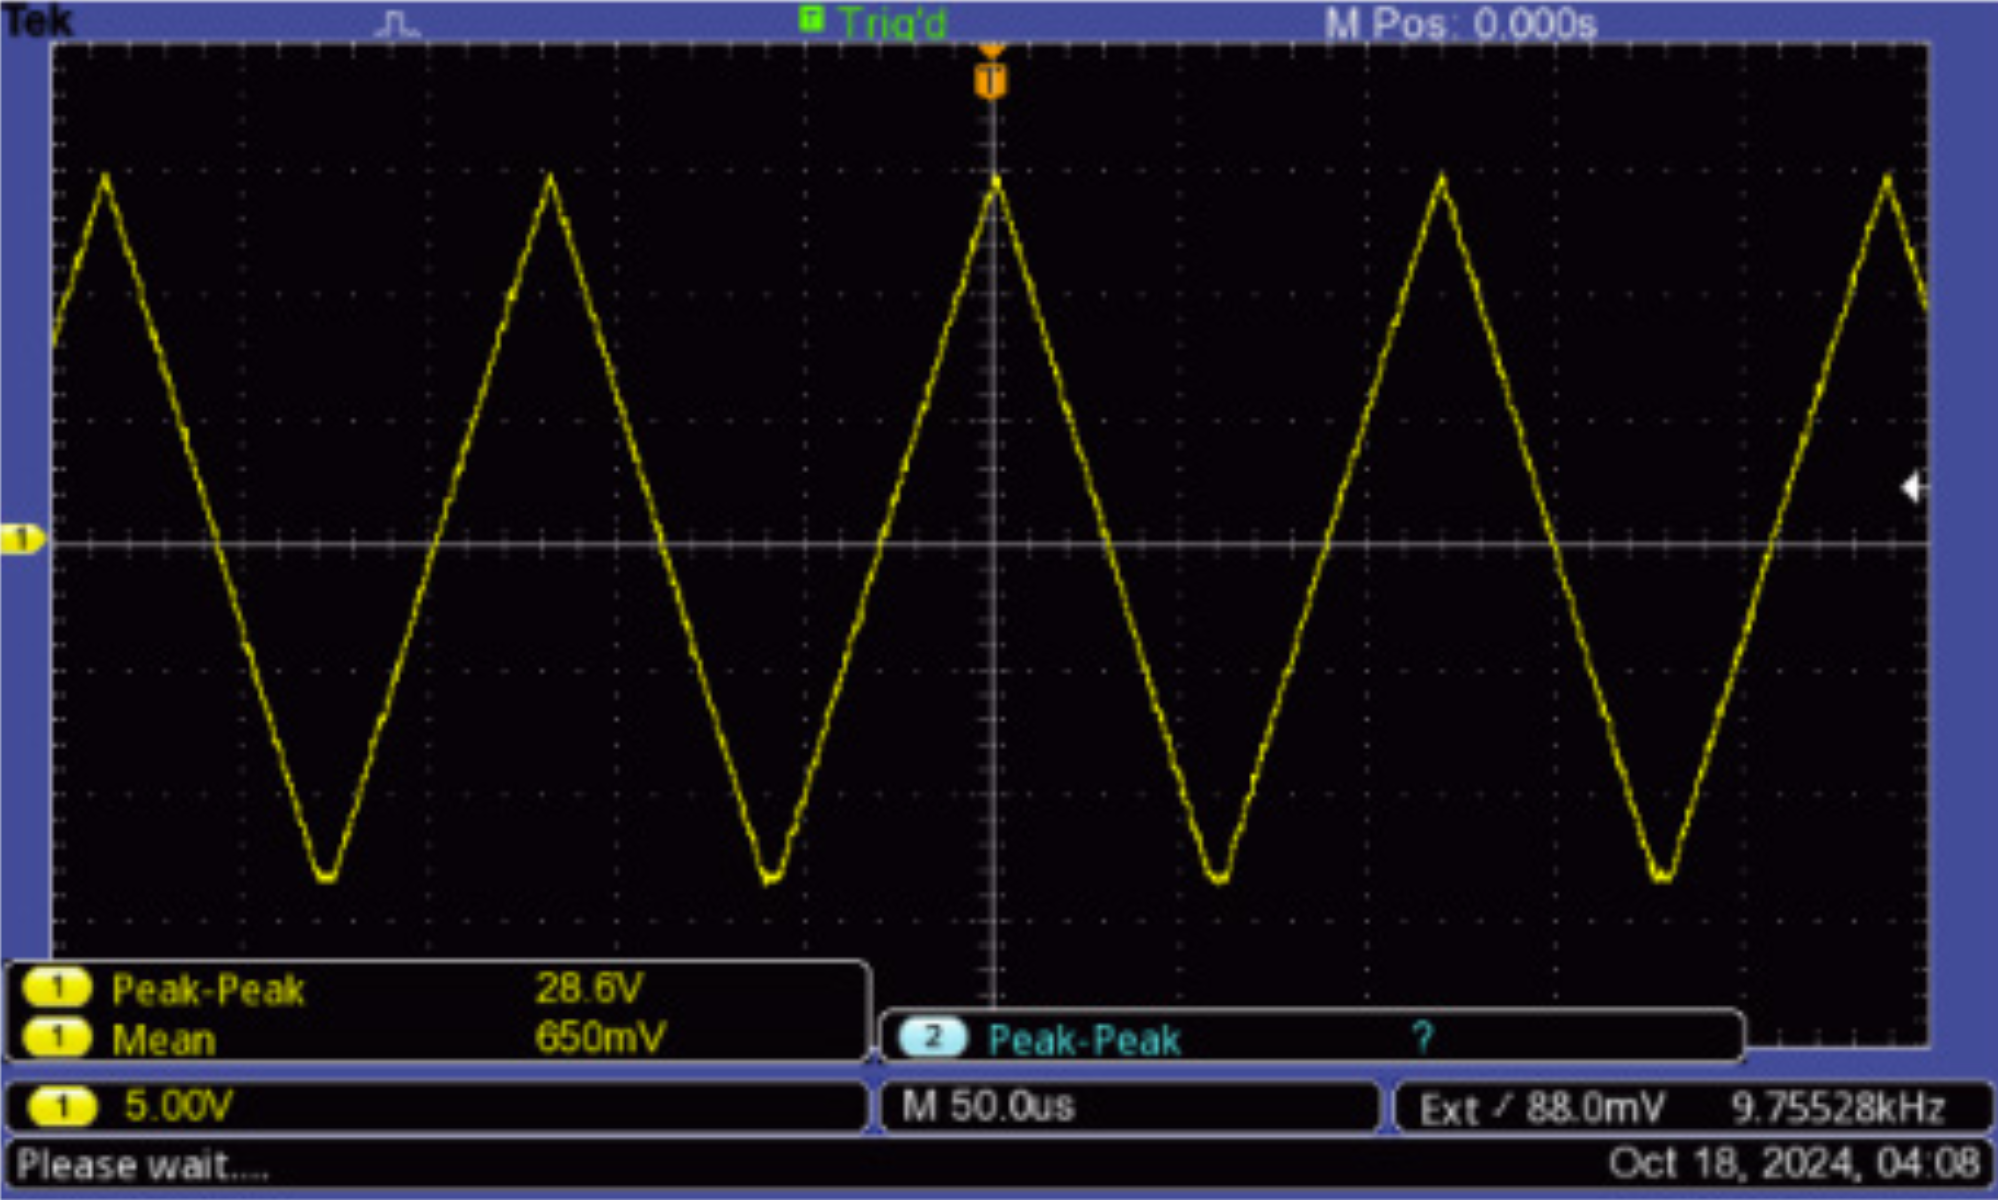
\includegraphics[width=0.8\textwidth]{img/Lab 8/1_3.png} % Replace with actual image
    \caption{}
\end{figure}

\begin{figure}[H]
    \centering
    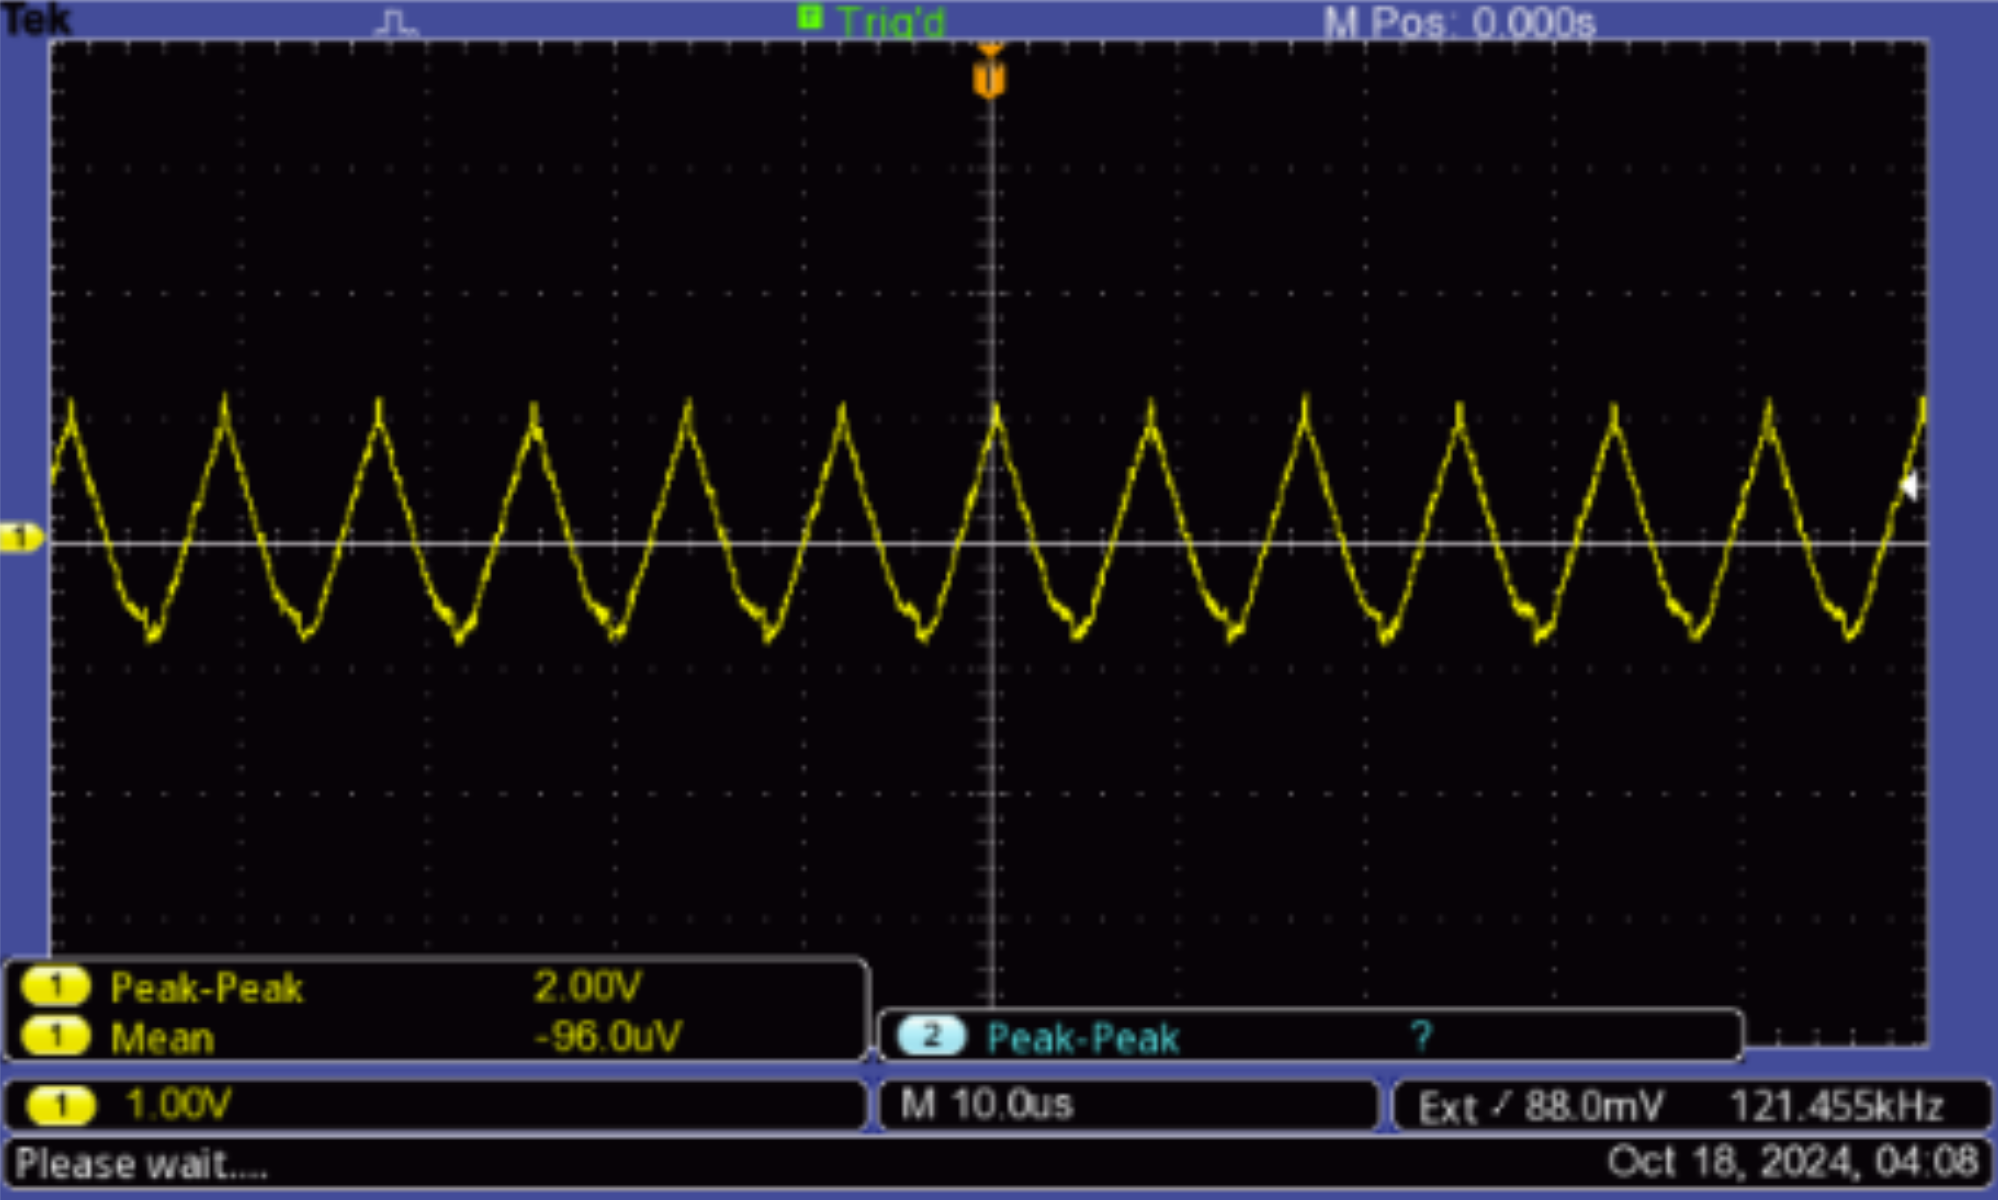
\includegraphics[width=0.8\textwidth]{img/Lab 8/1_4.png} % Replace with actual image
    \caption{}
\end{figure}

\begin{figure}[H]
    \centering
    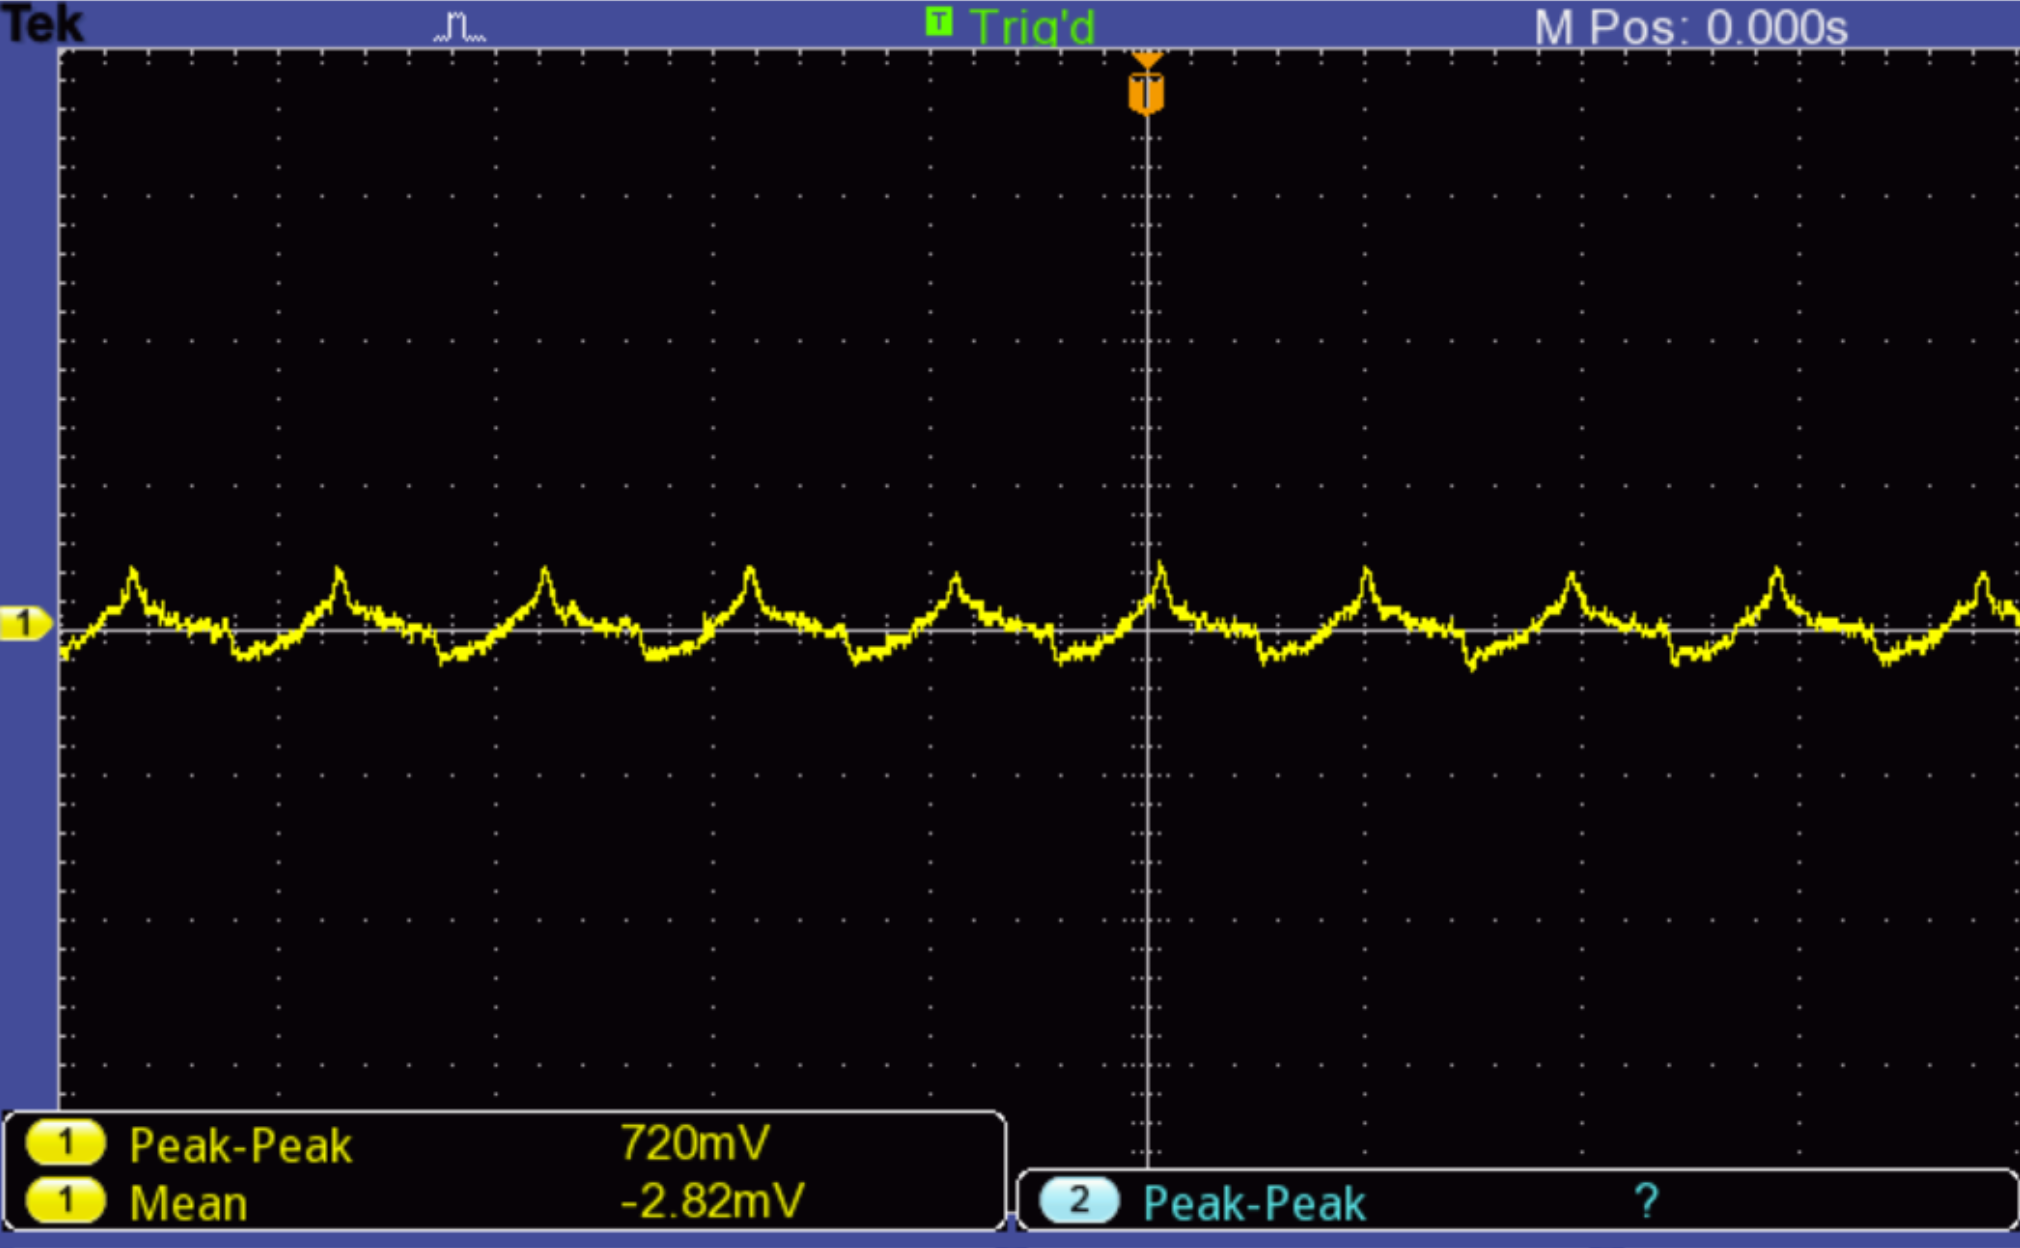
\includegraphics[width=0.8\textwidth]{img/Lab 8/1_5.png} % Replace with actual image
    \caption{}
\end{figure}

\\ \\ 

\subsection*{Question 2}

Using our knowledge of RC circuits, as well as the op-amp rules:

\begin{enumerate}
    \item The output attempts to do whatever is necessary to make the voltage difference between the two inputs zero.
    \item The inputs draw no current.
\end{enumerate}

We can derive the relationship between the input and output of the integrator as follows:

Since no current flows through the inputs, \( I_{\text{in}} \) does not split, so \( I_C = I_R \). Using Ohm’s law:

\[
I_R = \frac{V_{R_{\text{in}}}}{R_{\text{in}}} \quad \text{where} \quad V_{R_{\text{in}}} = V_{\text{in}} - V^-
\]

This simplifies to:

\[
I_R = \frac{V_{\text{in}} - V^-}{R_{\text{in}}}
\]

Using rule (2), \( V^- \) equals 0, acting as a virtual ground, so:

\[
I_R = \frac{V_{\text{in}}}{R_{\text{in}}}
\]

The capacitor current \( I_C \) is given by:

\[
I_C = C \frac{dV_{\text{out}}}{dt}
\]

Since \( I_C = I_R \), we have:

\[
C \frac{dV_{\text{out}}}{dt} = \frac{V_{\text{in}}}{R_{\text{in}}}
\]

Integrating both sides with respect to time:

\[
V_{\text{out}} = \frac{1}{R_{\text{in}}C} \int V_{\text{in}} \, dt
\]

Compared to an RC filter, an op-amp requires a stable \( V_{\text{in}} \) or power supply, while an RC filter is dependent on having a proper capacitor as it charges over time.

For the output magnitudes, an op-amp is constrained by the limits of the positive and negative rails, whereas an RC filter is constrained by the current voltage charge of the capacitor.


\subsection*{Question 3}
Using the following components: 
\( R_1 = 10\,\text{k}\Omega \), \( R_2 = 2\,\text{k}\Omega \), \( V_{CC} = +15\,\text{V} \), 
and \( V_{\text{in}} \) as a \( 4\,\text{V} \) peak-to-peak sine wave with no DC offset, 
we applied an external DC voltage source for \( V_{\text{DC}} \). We varied \( V_{\text{DC}} \) 
between 0 and 5.5\,V, observing \( V_{\text{out}} \) on the oscilloscope.
\\ 
\\

\begin{figure}[H]
    \centering
    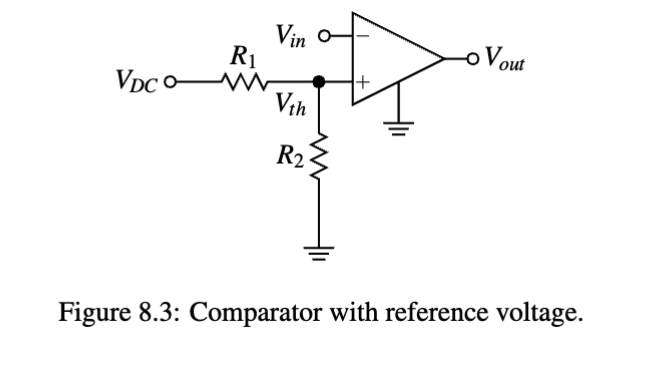
\includegraphics[width=0.8\textwidth]{img/Lab 8/3_1.png} % Update with the actual image path
    \caption{}
\end{figure}
\\

The waveforms below illustrate our observations. At \( V_{\text{DC}} = 5.5\,\text{V} \), 
the threshold voltage \( V_{\text{th}} \) exceeds the amplitude of \( V_{\text{in}} \). 
In the waveforms, \( V_{\text{in}} \) is shown in blue, while \( V_{\text{out}} \) 
and \( V_{\text{th}} \) are represented in yellow. The left set of waveforms displays 
\( V_{\text{out}} \) versus \( V_{\text{in}} \), while the right set shows \( V_{\text{th}} \) 
versus \( V_{\text{in}} \).

\begin{figure}[H]
    \centering
    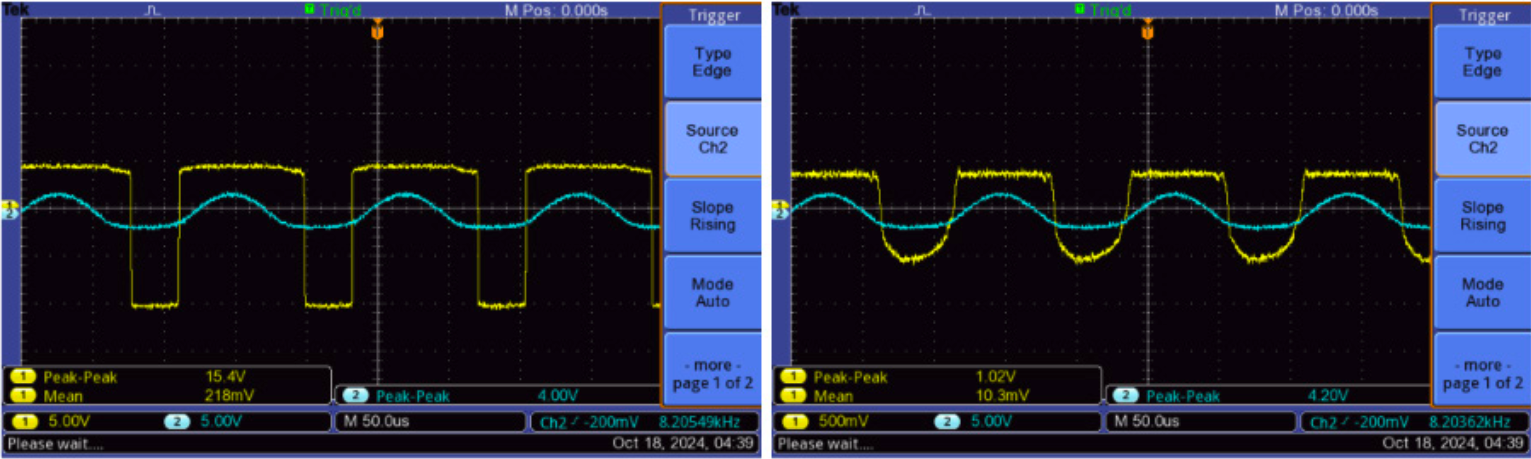
\includegraphics[width=0.8\textwidth]{img/Lab 8/3_2.png} % Update with the actual image path
    \caption{ \( V_{\text{DC}} = 0\,\text{V} \) }
\end{figure}

\begin{figure}[H]
    \centering
    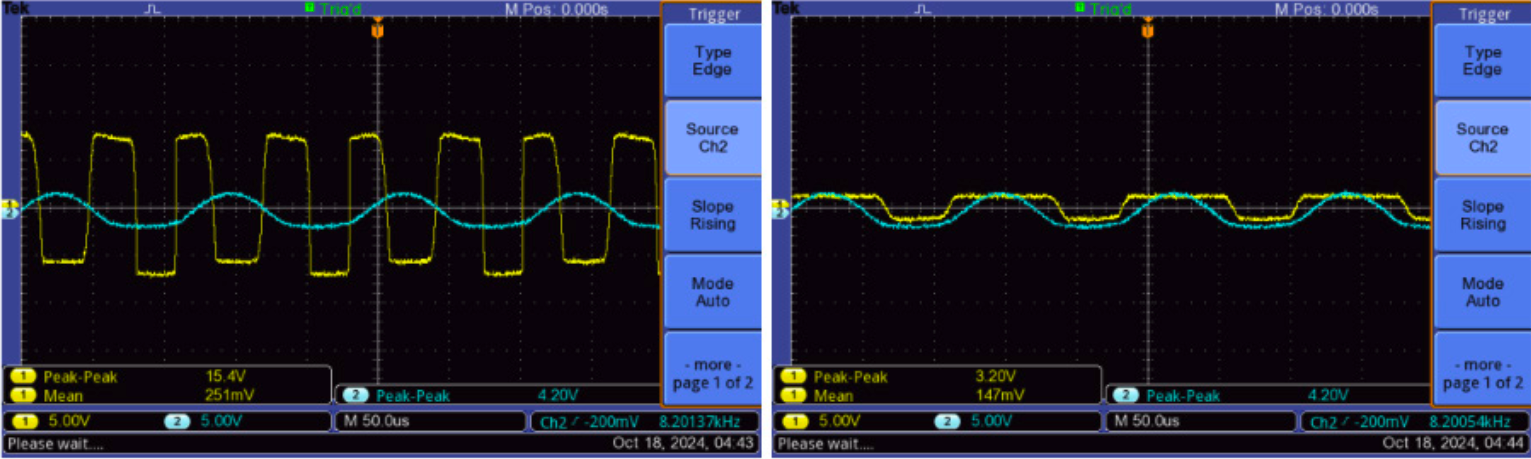
\includegraphics[width=0.8\textwidth]{img/Lab 8/3_3.png} % Update with the actual image path
    \caption{ \( V_{\text{DC}} = 5.5\,\text{V} \) }
\end{figure}

\begin{figure}[H]
    \centering
    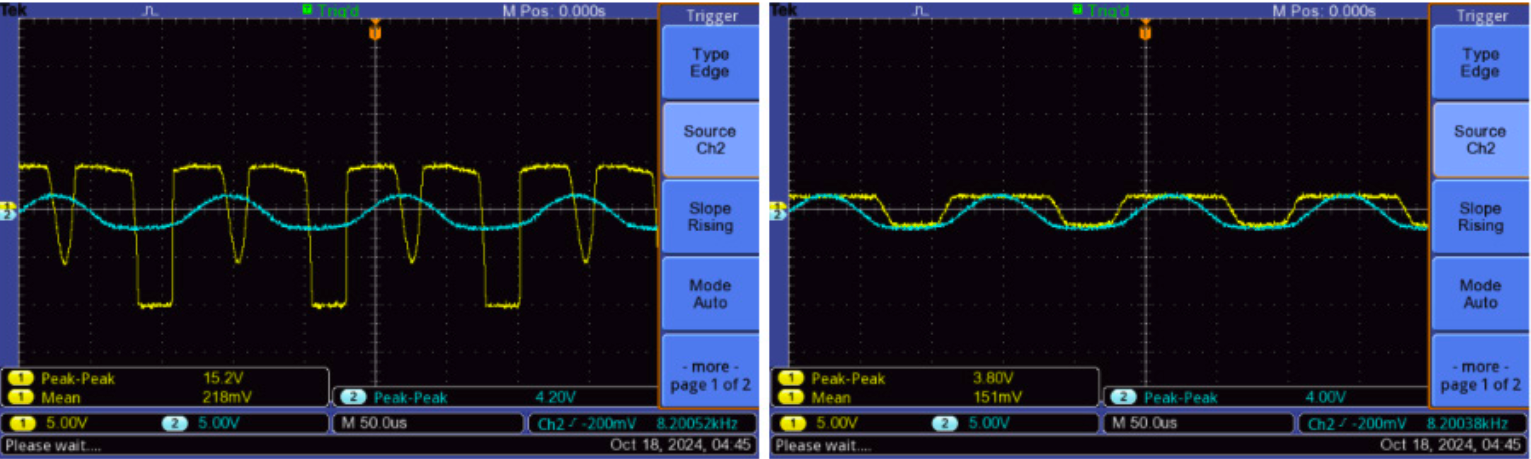
\includegraphics[width=0.8\textwidth]{img/Lab 8/3_4.png} % Update with the actual image path
    \caption{ \( V_{\text{DC}} = 2.3\,\text{V} \) }
\end{figure}

\begin{figure}[H]
    \centering
    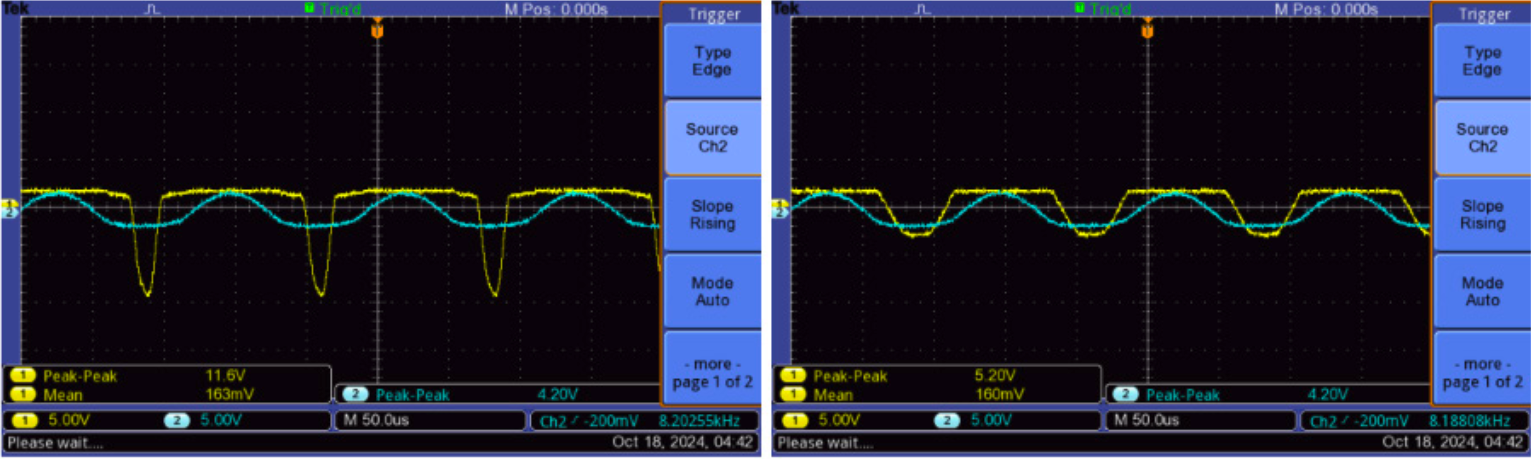
\includegraphics[width=0.8\textwidth]{img/Lab 8/3_5.png} % Update with the actual image path
    \caption{ \( V_{\text{DC}} = 3.2\,\text{V} \) }
\end{figure}

\subsection*{Explanation of Graphs}

\textbf{\( V_{\text{DC}} = 0\,\text{V} \):} 
At this setting, the output voltage \( V_{\text{out}} \) (yellow) switches between high and 
low levels, correlating with the zero-crossing points of the input sine 
wave \( V_{\text{in}} \) (blue). The threshold voltage \( V_{\text{th}} \) is 
relatively low, allowing the comparator to respond quickly to changes in \( V_{\text{in}} \).
\\

\textbf{\( V_{\text{DC}} = 5.5\,\text{V} \):}
Here, the threshold voltage \( V_{\text{th}} \) exceeds the amplitude of \( V_{\text{in}} \). 
This results in \( V_{\text{out}} \) switching states only when \( V_{\text{in}} \) 
crosses this higher threshold, causing less frequent transitions. This demonstrates how a 
higher \( V_{\text{DC}} \) delays the comparator's response, reducing switching frequency.
\\

\textbf{\( V_{\text{DC}} = 2.3\,\text{V} \):}
At this intermediate setting, \( V_{\text{th}} \) is higher than in the first case but 
lower than in the second. The switching frequency of \( V_{\text{out}} \) is also 
intermediate, showing delayed transitions compared to \( V_{\text{DC}} = 0\,\text{V} \), 
but more frequent than at \( V_{\text{DC}} = 5.5\,\text{V} \).
\\

\textbf{\( V_{\text{DC}} = 3.2\,\text{V} \):}
For this value, the threshold voltage is balanced, and the waveform behavior reflects the 
stable transition points based on the intermediate threshold voltage.
\\

\subsection*{Question 4}
In this experiment, we measured the upper and lower threshold voltages for 
the comparator circuit with and without the feedback resistor \( R_3 \).

\textbf{Without \( R_3 \):}
\begin{itemize}
    \item Lower threshold: \( 3.5\,\text{V} \, V_{\text{DC}} \)
    \item Higher threshold: \( 5.0\,\text{V} \, V_{\text{DC}} \)
\end{itemize}

\textbf{With \( R_3 \):}
\begin{itemize}
    \item Lower threshold: \( 2.2\,\text{V} \, V_{\text{DC}} \)
    \item Higher threshold: \( 4.1\,\text{V} \, V_{\text{DC}} \)
\end{itemize}

The following graphs illustrate the observed waveforms for both cases:

\begin{figure}[H]
    \centering
    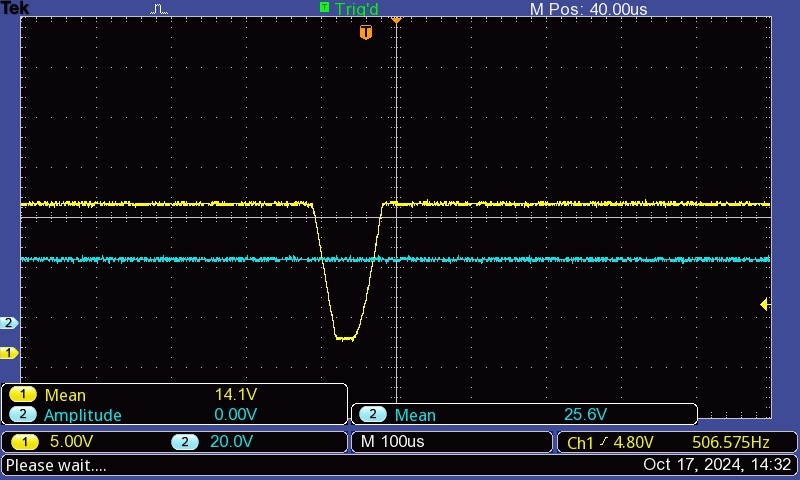
\includegraphics[width=0.8\textwidth]{img/Lab 8/noR_High.JPG} % Replace with "F0003TEK.JPG"
    \caption{Without \( R_3 \): Low Threshold (\( V_{\text{th}} = 3.5\,\text{V} \))}
\end{figure}

\begin{figure}[H]
    \centering
    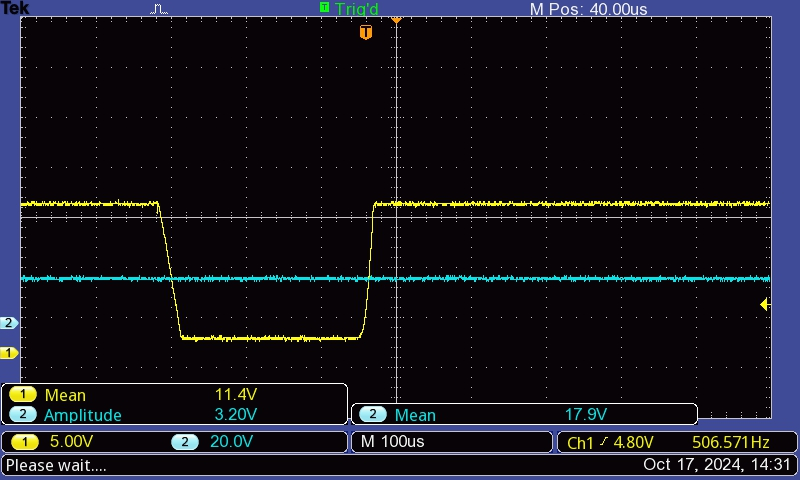
\includegraphics[width=0.8\textwidth]{img/Lab 8/noR_Low.JPG} % Replace with "F0004TEK.JPG"
    \caption{Without \( R_3 \): High Threshold (\( V_{\text{th}} = 5.0\,\text{V} \))}
\end{figure}

\begin{figure}[H]
    \centering
    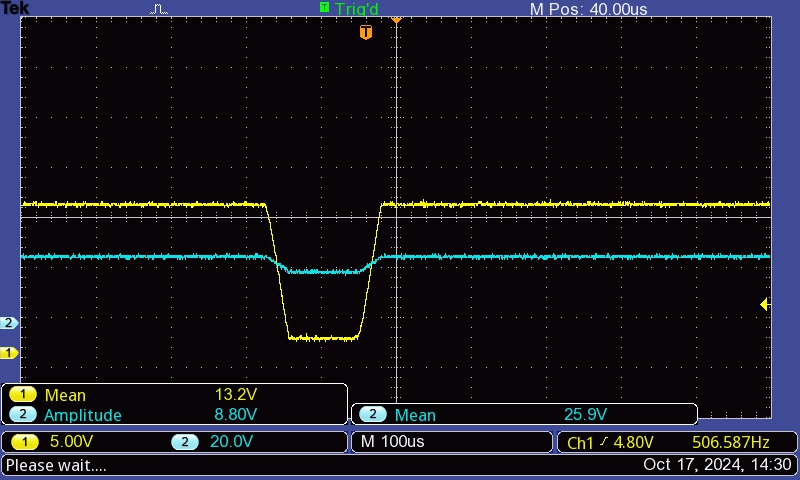
\includegraphics[width=0.8\textwidth]{img/Lab 8/R_High.JPG} % Replace with "F0005TEK.JPG"
    \caption{With \( R_3 \): Low Threshold (\( V_{\text{th}} = 2.2\,\text{V} \))}
\end{figure}

\begin{figure}[H]
    \centering
    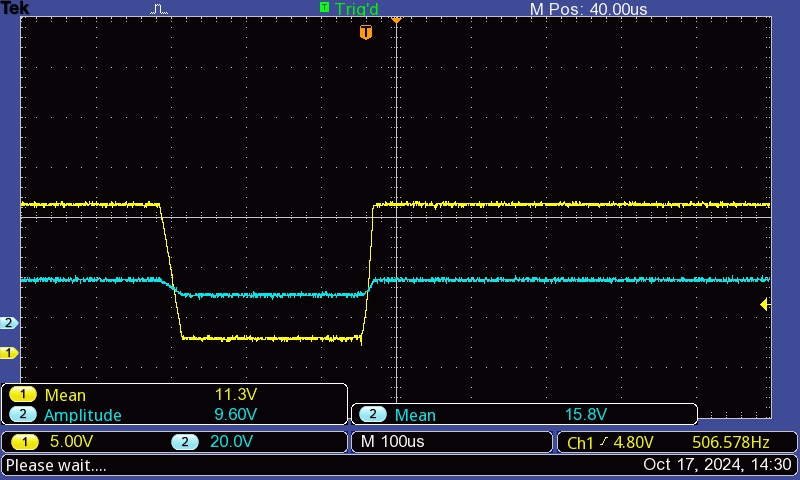
\includegraphics[width=0.8\textwidth]{img/Lab 8/R_Low.JPG} % Replace with "F0006TEK.JPG"
    \caption{With \( R_3 \): High Threshold (\( V_{\text{th}} = 4.1\,\text{V} \))}
\end{figure}

\subsection*{Explanation of Graphs}

\textbf{Without \( R_3 \):}

\begin{itemize}
    \item \textbf{Low Threshold (\( V_{\text{th}} = 3.5\,\text{V} \)):} \\
    The comparator switches its output state when the input voltage \( V_{\text{in}} \) crosses the lower threshold of \( 3.5\,\text{V} \). In the graph, \( V_{\text{out}} \) (yellow) transitions from high to low as \( V_{\text{in}} \) (blue) falls below this threshold. Without feedback, the switching is sharp and immediate, with no hysteresis present.
    
    \item \textbf{High Threshold (\( V_{\text{th}} = 5.0\,\text{V} \)):} \\
    Similarly, \( V_{\text{out}} \) switches from low to high when \( V_{\text{in}} \) exceeds the upper threshold of \( 5.0\,\text{V} \). In the graph, we see a sharp transition as \( V_{\text{in}} \) crosses the threshold. The absence of hysteresis results in straightforward switching behavior.
\end{itemize}

\textbf{With \( R_3 \):}

\begin{itemize}
    \item \textbf{Low Threshold (\( V_{\text{th}} = 2.2\,\text{V} \)):} \\
    Introducing the feedback resistor \( R_3 \) shifts the lower threshold to \( 2.2\,\text{V} \). The output \( V_{\text{out}} \) (yellow) switches from high to low only when \( V_{\text{in}} \) (blue) drops below this threshold. The hysteresis stabilizes the output, reducing sensitivity to noise and preventing frequent switching.
    
    \item \textbf{High Threshold (\( V_{\text{th}} = 4.1\,\text{V} \)):} \\
    The feedback reduces the upper threshold to \( 4.1\,\text{V} \). \( V_{\text{out}} \) switches from low to high when \( V_{\text{in}} \) exceeds this threshold. The hysteresis introduces a “dead zone” between the two thresholds, enhancing noise immunity and reducing unnecessary toggling.
\end{itemize}

\textbf{Summary:} \\
Without \( R_3 \), the comparator switches states sharply at the lower (\( 3.5\,\text{V} \)) and upper (\( 5.0\,\text{V} \)) thresholds, making it susceptible to noise. With \( R_3 \), hysteresis is introduced, shifting the thresholds to \( 2.2\,\text{V} \) and \( 4.1\,\text{V} \). This stabilizes the output, prevents rapid toggling, and improves performance in noisy environments by creating a memory effect.

\subsection*{Question 5}
Using the same circuit as above with \( R_3 \) connected, we observed the hysteresis curve directly by connecting both the input and output of the circuit to the oscilloscope in XY mode. Channel 1 (horizontal axis) displayed the triangle wave input \( V_{\text{in}} \), and Channel 2 (vertical axis) displayed the output \( V_{\text{out}} \).
\\
\\
Initially, we observed the hysteresis curve using a triangle wave input with no DC offset. As we varied the DC offset, we noted the following behavior: \\ 
- When increasing the DC offset positively, the bottom line of the hysteresis loop was displayed. \\
- When decreasing the DC offset negatively, the top line of the hysteresis loop appeared. \\

\\
This behavior shows that the hysteresis curve depends on the input signal's relationship to the threshold voltages. Below are the screenshots from the oscilloscope in XY mode, illustrating the hysteresis behavior.

\begin{figure}[H]
    \centering
    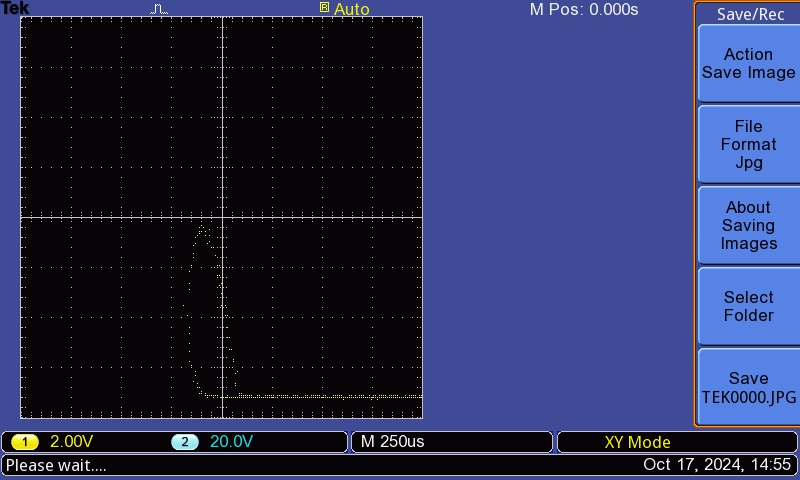
\includegraphics[width=0.8\textwidth]{img/Lab 8/5_1.JPG} % Replace with actual image path
    \caption{Hysteresis curve showing the bottom line when the DC offset is increased positively.}
\end{figure}

\begin{figure}[H]
    \centering
    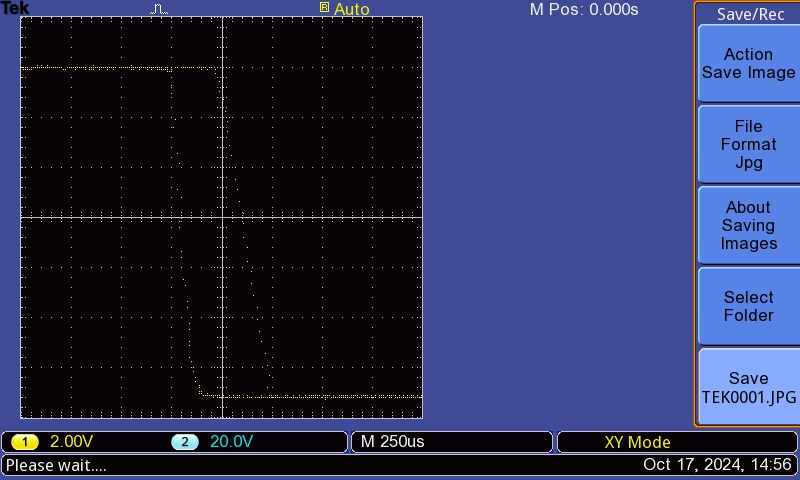
\includegraphics[width=0.8\textwidth]{img/Lab 8/5_2.JPG} % Replace with actual image path
    \caption{Hysteresis curve showing the top line when the DC offset is decreased negatively.}
\end{figure}

\textbf{Explanation:} \\
In XY mode, the hysteresis loop provides a visual representation of the 
input-output relationship of the Schmitt trigger. The curve shows how the 
output \( V_{\text{out}} \) changes state at different input voltages 
\( V_{\text{in}} \) due to the feedback resistor \( R_3 \), which introduces 
hysteresis. By varying the DC offset, we could observe how the hysteresis 
loop behaves, highlighting the switching behavior of the comparator circuit. 
We see this loop on the graph as the input signal moves between the upper 
and lower thresholds, demonstrating the memory effect of the Schmitt trigger.


\subsection*{Question 6}

Using our knowledge of RC circuits, as well as the op-amp rules:
\begin{enumerate}
    \item The output attempts to do whatever is necessary to make the voltage difference between the two inputs zero.
    \item The inputs draw no current.
\end{enumerate}

We can relate \( V_{\text{th}} \), \( V_{\text{DC}} \), \( V_{\text{out}} \), \( R_1 \), \( R_2 \), and \( R_3 \) in a single equation. According to Kirchhoff's law, the voltage at \( V_{\text{th}} \) equals \( V^+ \). Therefore, we can write:
\[
I_1 = \frac{V_{\text{DC}} - V_{\text{th}}}{R_1}, \quad I_2 = \frac{V_{\text{th}}}{R_2}, \quad I_3 = \frac{V_{\text{out}} - V_{\text{th}}}{R_3}
\]

From rule (1), we know that \( I_1 + I_3 = I_2 \).

Substituting our current formulas into the above equation, we get:
\[
\frac{V_{\text{DC}} - V_{\text{th}}}{R_1} + \frac{V_{\text{out}} - V_{\text{th}}}{R_3} = \frac{V_{\text{th}}}{R_2}
\]

After simplifying, we derive the following equation for \( V_{\text{th}} \):
\[
V_{\text{th}} = \frac{R_2 R_3 V_{\text{DC}} + R_1 R_2 V_{\text{out}}}{R_1 R_2 + R_1 R_3 + R_2 R_3}
\]

Using this equation, we can predict the threshold voltages from above. With \( V_{\text{DC}} = 10\,\text{V} \) and \( V_{\text{out}} \) at its maximum (\( \approx 15\,\text{V} \)), we calculate the threshold for \( V_{\text{out}} \) to transition away from its maximum as \( V_{\text{in}} = 4.52\,\text{V} \). This is close to our measured maximum threshold voltage of \( 4.96\,\text{V} \).

At \( V_{\text{out}} \) minimum (\( \approx 1.5\,\text{V} \)), using the formula for \( V_{\text{th}} \), we find the transition occurs at \( V_{\text{in}} = 2.89\,\text{V} \), which aligns closely with our measured minimum threshold voltage of \( 2.80\,\text{V} \).

A Schmitt trigger swaps \( V_{\text{out}} \) between high and low voltages, exhibiting hysteresis. This means the threshold for switching from low to high voltage (\( V_{\text{th}-} \)) is lower than the threshold for switching from high to low voltage (\( V_{\text{th}+} \)). Hysteresis helps prevent noise from causing random transitions, as significant changes in \( V_{\text{in}} \) are required to switch \( V_{\text{out}} \) back to its original state.

The hysteresis in a Schmitt trigger arises from positive feedback through \( R_3 \). When \( V_{\text{out}} \) is high, \( V_{\text{th}} \) increases, raising the threshold voltage. Conversely, when \( V_{\text{out}} \) is low, \( V_{\text{th}} \) decreases, lowering the threshold voltage. This behavior stabilizes the circuit by preventing rapid toggling due to minor input fluctuations.

The mathematical reasoning is derived from rule (2), which ensures no current is drawn by the inputs. Rule (1) explains why \( V^+ \) is equal to \( V^- \), leading to the observed switching behavior and the variation in \( V_{\text{th}} \) with \( V_{\text{in}} \).


\subsection*{Question 7}

For the final part of this lab, we were asked to construct the circuit shown in Figure 8.5, a relaxation oscillator using a TL071 op-amp.

\begin{figure}[H]
    \centering
    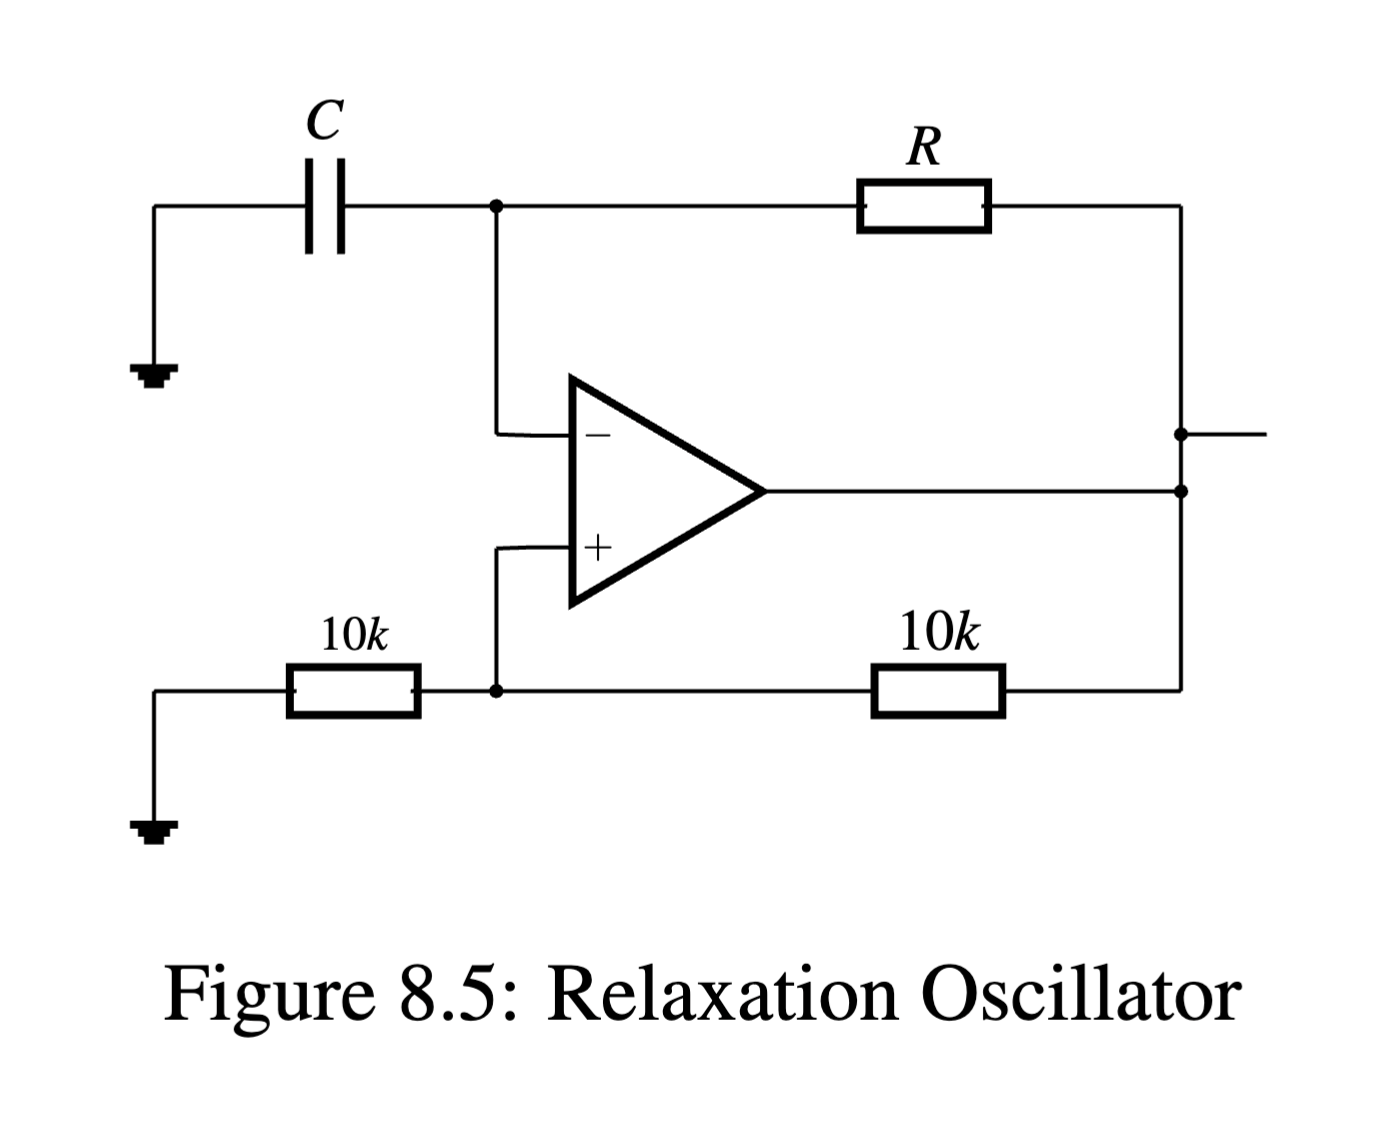
\includegraphics[width=0.5\textwidth]{img/Lab 8/7_1.png} % Replace with actual image path for the circuit diagram
    \caption{Relaxation Oscillator Circuit}
\end{figure}

We varied the resistor \( R \) and capacitor \( C \) components and recorded the oscillations using an oscilloscope. The component values of \( R \) and \( C \), along with the frequency of the resulting oscillation, are summarized in the table below.

\begin{table}[H]
    \centering
    \begin{tabular}{|c|c|c|}
        \hline
        \( C \, (\text{nF}) \) & \( R \, (\text{k}\Omega) \) & \( f \, (\text{kHz}) \) \\
        \hline
        1.0  & 161   & 2.22 \\
        10.5 & 161   & 0.216 \\
        3.36 & 161   & 0.684 \\
        3.36 & 20.1  & 6.24  \\
        3.36 & 44.3  & 2.89  \\
        10.5 & 44.3  & 0.913 \\
        10.5 & 20.1  & 2.03  \\
        1.0  & 44.3  & 9.14  \\
        1.0  & 20.1  & 19.6  \\
        \hline
    \end{tabular}
    \caption{Recorded values of \( C \), \( R \), and the resulting oscillation frequency \( f \)}
\end{table}

From our data, we observed that the output frequency is inversely proportional to the product of \( R \) and \( C \). In other words, the relationship can be described by the equation:
\[
f = \frac{1}{RC}
\]
This confirms the theoretical behavior of a relaxation oscillator, where the oscillation frequency depends on the time constant \( RC \).

`'
\section*{Lab 9: Operational Amplifiers III}

\end{document}
